\documentclass{anvil-paper}
\usepackage{array}
\usepackage{float}
\newcommand{\Nm}{\mathrm{N\,m}}
\newcommand{\dd}{\,\mathrm{d}}
\title{Adjoint Gradients for Torque-Ripple Optimization\\of a Nonlinear Motor}
\author{Robb Walters\\
  {\normalsize 2AM Logic}
  \and Crutcher Dunnavant\\
  {\normalsize ZSpaceLabs.ai}}
\date{October 2026\\[0.5ex]
  {\normalsize DOI: \href{https://doi.org/10.5281/zenodo.23580548}{10.5281/zenodo.23580548}}}
\hypersetup{pdftitle={Adjoint Gradients for Torque-Ripple Optimization of a Nonlinear Motor},pdfauthor={Robb Walters, Crutcher Dunnavant},pdfsubject={Matched optimization, torque-ripple reproduction and discrete design-gradient verification}}

\begin{document}
\maketitle
\begin{abstract}
A design gradient pays off only if it shortens the path to a validated
design. We reconstruct a published nonlinear
permanent-magnet motor in our GEODE finite-element code and minimize its
torque ripple over 8 or 18 shape parameters. The optimizers query a coarse
simulation; each new best design is rescored on a finer validation
simulation that no optimizer sees, and only validated scores count. Cost is
whole-run wall time on one single-threaded core per run. In a
preregistered, budget-matched study, SLSQP with adjoint gradients beat the
derivative-free COBYQA at the same coarse resolution in all 45 of the 50
paired comparisons where both succeeded, by geometric means of 3.10 and
7.79 at the primary targets, 90\% and 99\% reductions of the ripple
objective with 8 and 18 parameters. Two post-hoc ablations, under
protocols frozen beforehand, kept SLSQP but used forward differences,
splitting that advantage into a gradient factor and an optimizer factor.
The adjoint reached the primary target 1.71 and 2.70 times sooner, from
every start, than warm-started stencils, and 2.47 and 4.11 times sooner
than cold-started ones; COBYQA against
finite-difference SLSQP contributes the remaining 1.2 to 1.8 with 8
parameters and 1.9 to 2.9 with 18. The adjoint cuts the gradient's share
of the time to target from 45--77\% to about 5\%, so validation and
coarse forwards bound the end-to-end gain. Every target crossing
selected for final checks, 25 of the main study's 111 and 10 in each
ablation, kept its target on a finer mesh.
\end{abstract}

\section{Introduction}
Whether to pay for derivatives is a practical design decision. An adjoint
gives the sensitivities of a few outputs to many parameters for a cost
that does not grow with the number of parameters, whereas a
finite-difference gradient needs one extra solve per parameter
\citep{giles2000introduction,martins2013review}. That does not settle
whether following adjoint gradients reaches a good design sooner than a
derivative-free search or a cheaper gradient, or whether the design
survives a better model: the adjoint differentiates the chosen discrete
model and excitation policy. In aerodynamic shape optimization an adjoint
gradient-based method has needed far fewer function evaluations than a
genetic algorithm \citep{zingg2008comparative}, so the direction of an
advantage is expected. Its size for a nonlinear motor, measured on a
validated target with failures retained, is the question here.

We answer it in two steps. A preregistered, budget-matched study compares
five methods in two nested design spaces of a published nonlinear
permanent-magnet motor \citep{wiesheu2024spline}, judges every candidate
on one validation simulation, finer than any coarse simulation an optimizer
queries, and charges
whole-run wall time with nothing subtracted (Section~\ref{sec:optimization}).
There SLSQP with adjoint gradients beats COBYQA, but the contrast changes
the search strategy and the gradient together. Two post-hoc ablations
therefore keep SLSQP and replace the adjoint by forward differences
(Section~\ref{sec:exp2-fd}), so that the main contrast factors into a
gradient factor (finite-difference SLSQP against adjoint SLSQP) and an
optimizer factor (COBYQA against finite-difference SLSQP).
Table~\ref{tab:decomp} gives the main result. On one core per run, with the
stencil solved serially, the gradient factor is 1.71--2.47 with eight
parameters and 2.68--4.10 with 18, and the optimizer factor is
1.22--1.76 and 1.91--2.92. The range in each factor is the gap between the
two finite-difference baselines: stencil solves warm-started from the base
point's solution (FD-warm) or started from zero (FD-cold). The gradient
factor is set by the cost of the gradient, since all SLSQP arms cross each
primary target after the same number of validated designs, and it is
bounded by the time all arms spend on validation and coarse forwards
(Fig.~\ref{fig:decomp}).

Two checks make these measurements interpretable. The ripple objective
depends on the rotor--stator interface model: truncating harmonic coupling
at the reference's order 45 changes loaded ripple by 7--9\% and cogging by
59\% on the finest mesh, so the study validates at order 93
(Section~\ref{sec:model}). The design gradients pass finite-difference and
Taylor checks, yet verified ripple sensitivities differ between
interface/estimator models, and the excitation rule reverses mean-torque
sensitivities (Section~\ref{sec:gradients}). The numerical methods are
established; the contribution is the measured time-to-target evidence for
adjoint gradients, separated from the choice of optimizer, with the checks
that show what the gradients represent. Section~\ref{sec:discussion} states
what transfers.

\section{Related work}
\citet{wiesheu2024spline} combine spline-based rotor and stator shape
optimization with engineering parameters for a nonlinear permanent-magnet
synchronous motor, and their related study combines parameter and shape
optimization with isogeometric analysis \citep{wiesheu2025combined}. Their
public implementation and saved outputs provide the reproduction target.
We inherit the initial geometry, material table and excitation
conventions and replace the field discretization; the comparison is
between numerical models, not with a measured motor.

Adjoint shape sensitivity for nonlinear magnetostatics is long
established. \citet{park1992design} applied the adjoint variable method to
the finite-element equations of a saturated two-dimensional magnet design,
and \citet{elbechari2022adjoint} detail a discrete adjoint for linear and
nonlinear magnetostatics with geometric and physical variables, verified
against finite differences.
\citet{gangl2015shape} derive rotor shape sensitivities with a
shape-Lagrangian formulation to smooth the rotation pattern of a motor;
\citet{kuci2017design} derive shape sensitivities from the Lie derivative
and apply them to an interior permanent-magnet machine
\citep{kuci2016shape}. \citet{scotzniovsky2025} combine free-form
deformation, differentiable mesh warping and adjoint derivatives, and
\citet{merkel2021shape} use isogeometric shape derivatives with harmonic
rotor--stator coupling. \citet{martins2013review} review finite
differences, complex steps, algorithmic differentiation and direct and
adjoint methods in one framework, \citet{giles2000introduction} introduce
the adjoint approach to design, \citet{nikolova2004adjoint} review
adjoint-variable sensitivities for electromagnetic structure design, and
\citet{peter2010numerical} and \citet{kenway2019effective} survey
sensitivity-analysis approaches and adjoint practice for aerodynamic
optimization. These works establish why an adjoint gradient is cheaper than
a finite-difference one; Section~\ref{sec:exp2-fd} measures what that
saving is worth in time to a validated target. The accuracy of a
finite-difference gradient also depends on its step relative to the
function's computational noise, which \citet{more2011estimating} show how
to estimate and \citet{more2012estimating} use to choose a near-optimal
step; our finite-difference arms instead use one step fixed in advance.
For iteratively solved problems the perturbed solves' convergence error
enters as well: \citet{haftka1985sensitivity} gives a modified procedure
that improves such derivatives and \citet{eyi2011finite} chooses the step
from an estimate of that error, whereas our warm-started arm keeps the
frozen tolerance and reports the resulting error. The direct method, one
linearized solve per parameter \citep{adelman1986sensitivity}, and the
semi-analytic method, which can be inaccurate for shape variables
\citep{barthelemy1990accuracy}, lie between the two in cost; neither was
tested.

Interface order already matters for torque:
\citet{degersem2004harmonic} formulate harmonic weighting functions at the
sliding interface, \citet{bontinck2018isogeometric} use harmonic interface
constraints between isogeometric subdomains and analyze their stability,
and \citet{egger2022torque} derive torque from a harmonic mortar
formulation and vary the transmitted order in a linear cogging
experiment. We quantify its effect on loaded nonlinear ripple and design sensitivities,
using coupling torque and the gap-averaged stress of \citet{arkkio1987};
\citet{howe1992cogging} and \citet{arkkio2012proper} study discretization
effects on torque.

Optimizer benchmarks in machine design compare derivative-free methods:
\citet{duan2013review} compare response-surface and differential-evolution
search on a five-variable permanent-magnet motor, and
\citet{bramerdorfer2018modern} survey optimization practice for electrical
machines, and \citet{lei2017review} review their design-optimization
methods. \citet{ion2018robust} compare deterministic gradient-based and
stochastic search for electric devices. \citet{gangl2022multi} report
minutes for gradient-based free-form shape optimization of a synchronous
reluctance machine against hours for a stochastic parametric optimization
that found similar shapes, a comparison that also changes the
parametrization and the solver. \citet{zingg2008comparative}
found that a genetic algorithm needed 5 to 200 times as many function
evaluations as an adjoint method in aerodynamic shape optimization.
On an eight-variable wing twist problem, \citet{yu2018influence} found
gradient-free optimizers 4 times (NOMAD) to over 100 times (NSGA2, which
converged to a slightly worse design) as expensive as adjoint-driven ones,
the counterpart of our eight-parameter
SLSQP-against-COBYQA ratios of 3.10--3.25. They do not compare adjoint with
finite-difference gradients, which our ablation does, but state its premise:
finite-difference cost grows with the number of variables and adjoint cost does not. Our
time-to-target measure follows the performance profiles of
\citet{dolan2002benchmarking} and the data profiles of
\citet{more2009benchmarking}, with a wall-time budget and censored
targets.

\section{Motor model}\label{sec:model}
\subsection{Geometry and operating states}
The full machine has six poles and 36 stator slots. We model a
$60^\circ$ sector, polar angles $60^\circ$ to $120^\circ$ at zero
rotation, with antiperiodic conditions on the radial boundaries. The rotor
(radii 16 to 44\,mm) carries one buried permanent magnet per pole and
turns; the stator (radii 45 to 67.5\,mm) is fixed and carries the windings
in the slots between its teeth. Axial length is $L=0.1$\,m. The 1\,mm air
gap is split at the coupling radius $r_c=44.5$\,mm, where the separately
meshed rotor and stator meet. Figure~\ref{fig:geometry} shows the initial
design with its parts, the eight scalar design parameters and the 55
control points that the larger design space moves
(Section~\ref{sec:optimization}).

\begin{figure}[htbp]
\centering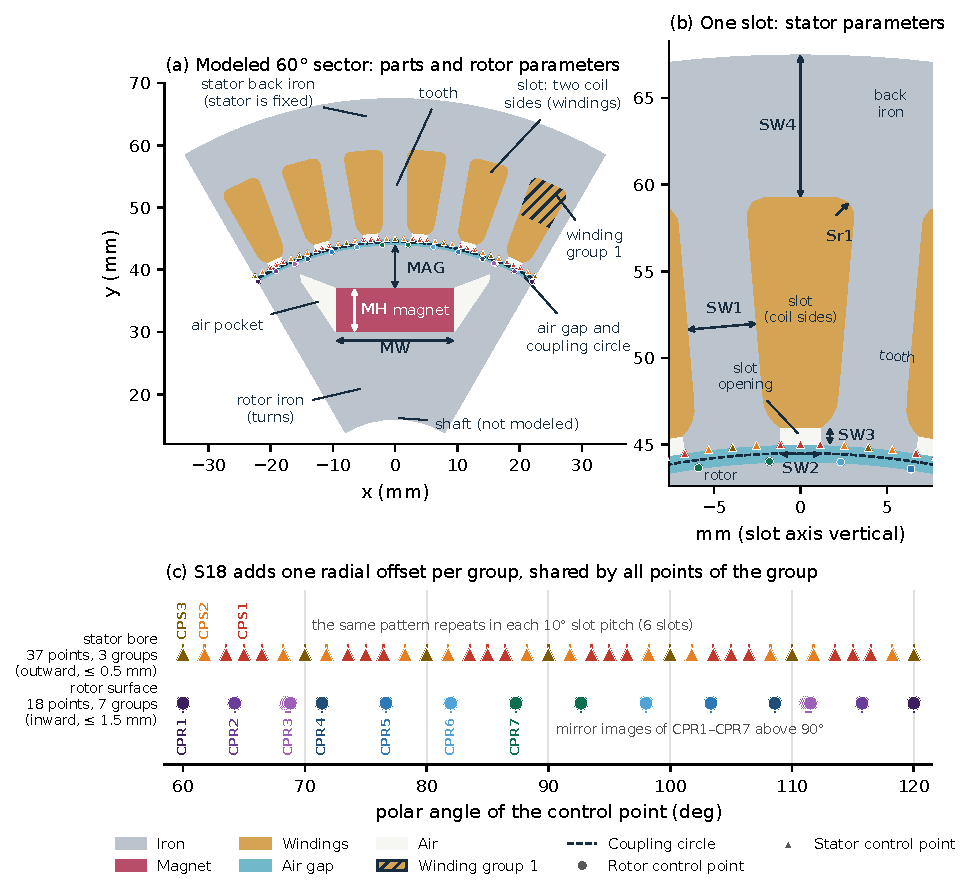
\includegraphics[width=\linewidth]{figures/geometry.pdf}
\caption{Initial design, rendered from the committed coarsest mesh
(element edges hidden). (a) The modeled sector and its parts, with the
rotor parameters: MAG, iron depth between the magnet and the rotor surface
on the pole axis; MH, magnet height; MW, magnet width. Winding group~1,
whose current density the reference optimizer holds fixed
(Section~\ref{sec:gradients}), is hatched. (b) One slot, turned so that its
axis is vertical, with the stator parameters: SW1, tooth width; SW2 and
SW3, width and depth of the slot opening; SW4, back-iron depth on the slot
axis; Sr1, radius of the fillets at the slot bottom. (c) The 55 control
points on the rotor surface and the stator bore, by polar angle. The
18-parameter space S18 adds ten offsets, one per group (CPR1--CPR7 on the
rotor, CPS1--CPS3 on the stator); an offset moves every point of its group
radially by the same distance, inward on the rotor (at most 1.5\,mm, 1\,mm
for CPR3) and outward on the stator (at most 0.5\,mm). Markers in (a) and
(b) use the colors of (c).}
\label{fig:geometry}
\end{figure}

The reference describes the geometry as NURBS patches, spline pieces
defined by weighted control points, and the reconstruction uses its initial
exports. Their control points are stored with weights already multiplied
in, and patch orientation must be accounted for when integrating areas. Two
thin rotor patches described as air slits in source comments receive iron
under the reference's material assignment; we follow that assignment. The
mesh generator, built on Gmsh 4.15.2 \citep{geuzaine2009gmsh}, keeps the
12 winding groups (the two coil sides of each slot) separate, since their
two characteristic areas are approximately 36.29 and 31.22\,mm$^2$.

At mechanical angle $\beta$, phase currents are
\begin{equation}
 I_q(\beta)=a I_*\sin(\phi_0+3\beta+\delta_q),\qquad
 (\delta_U,\delta_V,\delta_W)=(0,-2\pi/3,2\pi/3),
 \label{eq:current}
\end{equation}
where the current fraction $a\in\{0,0.5,1\}$ selects three operating
states (at $a=0$ only the magnets act; $a=0.5$ and $1$ are loaded),
$I_*=9.677657374$\,A, and the electrical phase offset $\phi_0=0$ for the
initial design. Angles in
Eq.~\eqref{eq:current} are in radians. Each winding group carries current
density $J_g=12s_g I_q/|\Omega_g|$, with its own area and prescribed sign
$s_g\in\{-1,1\}$. Using a common area would change the current density
between groups by about 16\%. We compare 20 distinct mechanical angles,
$0^\circ,1^\circ,\ldots,19^\circ$, excluding the duplicated endpoint in
the source CSV. The reference's optimization grid contains the ten even
angles; both grids are retained in the artifacts.

\subsection{Field model and rotor--stator coupling}
We solve two-dimensional nonlinear magnetostatics for the vector potential
$A_z$ with continuous piecewise-linear triangles and a tabulated M27 iron
law, using Newton's method with the consistent material tangent. The
separately meshed rotor and stator meet on the coupling circle, across
which the rotor mesh turns, in one of two ways. A conforming interface
identifies matching trace nodes after rotation. The harmonic model,
following the reference, matches the two sides only in the Fourier modes
of the field on that circle of orders $n=3,9,\ldots,N_h$, through Lagrange
multipliers, with $N_h=45$ unless stated otherwise. It passes only the
lower orders of the interface field, like a low-pass filter; a higher
interface order $N_h$ passes more of them, and the conforming interface
passes all that the mesh resolves. Torque is evaluated either by the
Arkkio expression, the Maxwell stress averaged over the air-gap annulus
\citep{arkkio1987}, or, for the harmonic model, by the coupling torque, the
derivative of the stored energy with respect to rotation through the
interface constraint \citep{egger2022torque}. Forward comparisons use Arkkio for both couplings
to isolate the interface change; the derivative study pairs harmonic
coupling with coupling torque and conforming coupling with Arkkio; the
optimization study's coarse simulation uses order-45 coupling torque and
its validation simulation order 93. Retaining every order below the trace Nyquist limit reproduces
the conforming Arkkio torques within $4.1\times10^{-9}$\,N\,m on L0 and
$1.3\times10^{-9}$\,N\,m on L1, without fitting any parameter to the saved
torque. Appendix~\ref{sec:fieldmodel} gives the weak form, tangent, iron
law, coupling constraints and torque expressions.

\subsection{Meshes and statistics}
The study uses four meshes, L0 (coarsest) to L3 (finest), with 3,153,
9,937, 36,083 and 139,268 nodes. The $60^\circ$ coupling arc has $120\cdot2^\ell$ segments at level
$\ell$, so integer-degree rotation is represented at every level.
A solution at one angle initializes the next angle at the same current.
We report the mean $\bar T$ and the population standard deviation
$\sigma_T$ of the torque over the $N=20$ angles; $\sigma_T$ is the ripple
metric. At zero current it measures
cogging, the torque variation caused by the permanent magnets and slots
without applied phase current. The squared-ripple objective is
$F=\sum_{a\in\{0,0.5,1\}}\sigma_T(a)^2$, in $\mathrm{N^2\,m^2}$, on the
20-angle grid. Torque ripple is a source of vibration and acoustic noise,
and the reference optimization minimizes it; because a design can also
lower ripple by giving up torque, the optimization study holds a floor on
the mean torque
(Section~\ref{sec:optimization}). Appendix~\ref{sec:fieldmodel} lists the
implementation checks.

\subsection{Interface order sets the validation simulation}\label{sec:coupling-results}
Table~\ref{tab:torque} compares the same geometry, material and excitation
with two interface models. The conforming L3 means are 0.15\% and 0.16\%
low at half and full current. Harmonic coupling reduces the mean deviations
to $-0.002\%$ and $+0.051\%$, with both reference means inside the estimated
refinement intervals. The loaded ripple deviations fall from $+9.9\%$
and $+11.3\%$ to $+1.7\%$ and $+1.3\%$.

\begin{table}[htbp]\centering\small
\caption{L3 population standard deviation and mean torque, in N\,m per
sector, on the 20-angle grid. The last column gives ripple deviation from the
saved reference; n/a identifies the reference itself. The reference is
subsequently refined in Section~\ref{sec:refinement}.}
\label{tab:torque}
\begin{tabular}{llrrr}\toprule
Current fraction & Model & Mean & Std & Std vs ref. (\%)\\\midrule
0 & Reference & 0.00010 & 0.01071 & n/a \\
0 & Conforming & 0.00001 & 0.00760 & $-$29.1 \\
0 & Harmonic & 0.00000 & 0.01209 & +12.9 \\
0.5 & Reference & 0.66208 & 0.03895 & n/a \\
0.5 & Conforming & 0.66106 & 0.04279 & +9.9 \\
0.5 & Harmonic & 0.66206 & 0.03961 & +1.7 \\
1 & Reference & 1.44248 & 0.07935 & n/a \\
1 & Conforming & 1.44023 & 0.08829 & +11.3 \\
1 & Harmonic & 1.44322 & 0.08036 & +1.3 \\
\bottomrule\end{tabular}

\end{table}

Spatial refinement at fixed order and order refinement on a fixed mesh
answer different questions (Fig.~\ref{fig:convergence}; Appendix~\ref{sec:forward} defines the refinement interval). At L3, order 45
raises cogging standard deviation by about 59\% and lowers loaded
standard deviation by 7--9\%, relative to the conforming values. At L1 and L2,
order 189 approaches the conforming torque to within $1.1\times10^{-4}$\,N\,m.
A spatially refined order-45 solution thus remains a solution of a
truncated interface model. Matching that truncation improves reproduction
of the published calculation; it does not establish which model better
represents the physical motor.

\begin{figure}[!t]\centering
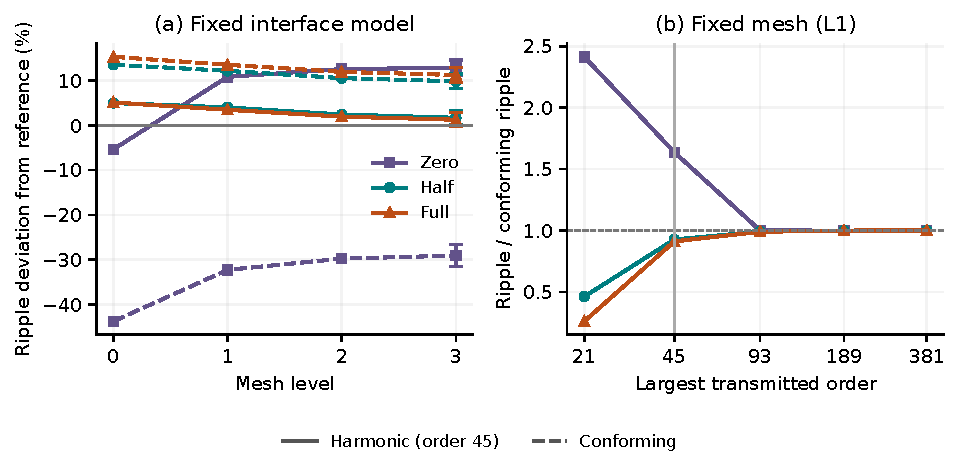
\includegraphics[width=.92\linewidth]{figures/coupling-convergence.pdf}
\caption{Left: ripple deviation from the reference under spatial
refinement, with solid lines for harmonic order 45 and dashed lines for
conforming coupling; L3 bars use Eq.~\eqref{eq:band}. Right: order
refinement on L1 with logarithmic order spacing, normalized by the
conforming ripple at that same level.
The saved reference uses order 45; see Section~\ref{sec:refinement} for its
refinement. Colors identify current, not coupling.}
\label{fig:convergence}\end{figure}

Rerunning the public reference with its own isogeometric model at four
refinement levels reduces its cogging discrepancy with GEODE from 12.9\%
to 0.10\%, so the coarse saved reference explains the initial cogging gap
at matched order, although neither refinement sequence is fully converged.
For the reference's saved optimized design (its iteration-120 design,
Opt120), raising the order from 45 to 93 multiplies its squared-ripple
objective by 3.6. Appendix~\ref{sec:forward}
gives these checks, the estimator and material controls, and the saved
design's size and current normalizations.

\section{Matched optimization study}\label{sec:optimization}
This section tests whether adjoint-driven optimization shortens the time
needed to reach a common validated ripple target. The protocol and all of
its amendments were fixed in the
\href{https://github.com/rjwalters/geode-fem/issues/1185}{preregistration}
before any main-run outcome was observed. One later deviation, in how the
final refinement was run, was adopted after the main runs had finished and
is described with the refinement in Section~\ref{sec:exp2-refinement}; it
changes no selection rule, check or target.

\subsection{Protocol}
\paragraph{Coarse and validation simulations.}
The optimizers never query the simulation that scores them. Each queries a
\emph{coarse simulation}, the L1 mesh (the coarser L0 for methods D and E)
with interface order 45, and its search is driven only by coarse values.
Every design that becomes the method's new best, its incumbent, is rescored
on one \emph{validation simulation}, the finer L2 mesh with interface order
93, which no optimizer sees; only validated scores count toward a target.
Unqualified, \emph{model} means a formulation of the simulation, such as the
field or interface model; no simulation is trained or fitted to torque data.
Of the models the optimizers use, only their own search models are fitted,
to coarse values: C's radial-basis surrogate and COBYQA's interpolation model.
Validation is charged to the run that requests it, as in a
design loop that must check its candidates before trusting them; this
validate-every-incumbent rule costs methods that change incumbents often
the most, and Section~\ref{sec:exp2-results} reports its share of each
run's time.

\paragraph{Methods.}
Five methods form an optimizer-by-resolution comparison plus one
surrogate (Table~\ref{tab:methods}). A and E are SLSQP
\citep{kraft1988} using the field adjoints of Section~\ref{sec:gradients},
safeguarded so that a refused request restores the last admissible point
and restarts the solver; B and D are COBYQA \citep{ragonneau2022} with $2n+1$ interpolation points
and unit-box trust radii $0.1$ to $10^{-6}$, where $n$ is the number of free
parameters. Both run through SciPy 1.18.1 \citep{virtanen2020scipy}. C is
an empirical trust-region method on four cubic radial-basis interpolants
of the L1 coarse outputs (the three per-current standard deviations and
the full-current mean), refitted after every evaluation from an $n+1$-point
initial design; Appendix~\ref{sec:settings} gives its radii, acceptance
and update rules and the other settings. A/B and E/D vary the optimizer at fixed coarse resolution,
and A/E and B/D vary resolution at fixed optimizer. The optimizer contrast
changes the search strategy and the gradient source together;
Section~\ref{sec:exp2-fd} separates them with the three further methods of
Table~\ref{tab:methods}. The coarse simulation uses order-45 coupling torque
on 20 angles at current fractions $0$, $\tfrac12$ and $1$ of the fixed peak
current $9.6777\,\mathrm{A}$. L0 and L1 differ only in spatial resolution,
and neither is fitted or corrected against validation. Time to a fixed
target, with unattained targets kept as censored, follows the data- and performance-profile
practice for benchmarking optimization solvers \citep{more2009benchmarking,dolan2002benchmarking}.
The preregistration also named a fixed group-1 current-density rule as a
labelled control. It was not run in this study, which uses the fixed
physical current throughout; Section~\ref{sec:gradients} reports that
rule's effect on sensitivities.

\begin{table}[H]\centering\small
\caption{Methods. A--E form the preregistered study (two repeats each).
FD-cold, FD-warm and A$'$ form the post-hoc ablations of
Section~\ref{sec:exp2-fd}; each ablation ran in its own session with A
rerun unchanged as A$'$. D and E solve the coarse nonlinear field
equations; they are neither fitted magnetic circuits nor reduced-basis
models.}
\label{tab:methods}\setlength{\tabcolsep}{5pt}
\begin{tabular}{llll}\toprule
Method & Optimizer or search model & Gradient & Optimization mesh\\\midrule
A & Safeguarded SLSQP & Field adjoint & L1\\
B & COBYQA & None & L1\\
C & Empirical cubic-RBF trust region & None & L1\\
D & COBYQA & None & L0\\
E & Safeguarded SLSQP & Field adjoint & L0\\\addlinespace
FD-cold & Safeguarded SLSQP & Forward differences, cold stencils & L1\\
FD-warm & Safeguarded SLSQP & Forward differences, warm stencils & L1\\
A$'$ & A, rerun in each ablation & Field adjoint & L1\\\bottomrule
\end{tabular}
\end{table}

\paragraph{Design spaces and constraints.}
The 8-parameter space S8 frees eight geometric lengths: MAG, MH, MW,
SW1--SW4 and Sr1 (Fig.~\ref{fig:geometry}a,b), that is, the rotor iron
depth, magnet height and width, four stator tooth and slot dimensions, and
the slot-bottom fillet radius. The 18-parameter space S18 adds the ten
grouped offsets of Fig.~\ref{fig:geometry}c, which move 55 control points
of the rotor surface and the stator bore. Stack length, radial scale,
stator outer diameter and operating angle are fixed, so the saved Opt120
design lies outside both spaces. Table~\ref{tab:paramsets} compares these
spaces with the 12-parameter set whose gradients Section~\ref{sec:gradients}
verifies. The two spaces also use different discrete mesh-motion maps, so
their contrast does not isolate the ten added offsets.
Each coarse simulation $r\in\{\mathrm{L0},\mathrm{L1}\}$ minimizes
$F_r=\sum_c\sigma_{r,c}^2$ over the three objective currents $c$, subject to
$\mu_{r,1}\geq1.0025\,\mu_{r,1}(\theta_0)$ for its own full-current mean and to
normalized construction margins $c_i-0.05\geq0$. Here $\theta_0$ is the
reference's published initial design. Unbuildable or
mesh-infeasible candidates are refused: SLSQP restores toward the last
admissible point and restarts, COBYQA receives a NaN barrier, and C skips
the point. A moved mesh with an inverted triangle or a minimum angle below
$5^\circ$ is repaired by up to four charged remeshing attempts. Because
refinement cannot remove a limiting geometric corner, the $5^\circ$ policy
also acts as an implicit geometric constraint. S18's slot-opening
channel wall is not guarded and can become very thin at extreme offsets;
that risk is handled by repair and refusal, not by a wall-thickness
constraint.

\begin{table}[H]\centering\small
\caption{The three parameter sets. Section~\ref{sec:gradients} verifies
the gradients of a 12-parameter scalar set; the optimizers search S8 and
S18, whose gradients are checked separately
(Appendix~\ref{sec:protocol-details}). Values are in
Table~\ref{tab:parameters}.}
\label{tab:paramsets}
\begin{tabular}{llll}\toprule
Parameters & Gradient check (12) & S8 & S18\\\midrule
MAG, MH, MW (magnet) & free & free & free\\
SW1--SW4, Sr1 (stator slot) & free & free & free\\
SD1, axial length, $\phi_0$, radial scale & free & fixed & fixed\\
CPR1--CPR7, CPS1--CPS3 (offsets) & --- & --- & free\\\bottomrule
\end{tabular}
\end{table}

The gradients A and E use, including those of S18's grouped offsets,
agree with central differences in both spaces within $2.8\times10^{-7}$
relatively in the directional checks (Appendix~\ref{sec:protocol-details}).

\paragraph{Common validation and credit.}
Every method is judged on the same order-93, L2, 20-angle validation simulation.
Its initial-design anchor is $F_0=9.6034\times10^{-3}\,\mathrm{N^2\,m^2}$ with
full-current mean $\mu_0=1.44084\,\Nm$. Target $T_x$ is an $x$\% reduction
of $F_0$: $T_{50}=0.5F_0$, $T_{90}=0.1F_0$ and $T_{99}=0.01F_0$. The
\emph{primary targets} are $T_{90}$ in S8 and $T_{99}$ in S18, the deepest
target reached in each space (no run reaches $T_{99}$ in S8). A validated
design is credited, and attains a target, only if
\begin{equation}
 F_{\mathrm{val}}+\delta F\leq T,\qquad
 \delta F=\max\{0.10F_{\mathrm{val}},\,2.5\times10^{-7}\,\mathrm{N^2\,m^2}\},
\end{equation}
its validated full-current mean is at least $1.0025\,\mu_0$, its
construction margins and mesh checks pass, and its validation completes
within budget. The allowance $\delta F$ is an empirical margin, not a bound
on continuum error. Optimizer success flags confer no credit. Changed
incumbents are validated as they appear, after the initial interpolation
set for B, C and D. A run's \emph{target crossing} is its first validated
design that attains the target; the time to the target is the charged time
at which that validation completes.

\paragraph{Budget, timing and cost vocabulary.}
Cost is wall time, in units of the median cold validation forward measured
on the same host at the same concurrency (66.66--70.94\,s in the three
sessions). A \emph{forward} is one evaluation of the objective: 60
nonlinear field solves, one per current fraction (3) and rotor angle (20).
In a \emph{cold} forward, Newton starts from zero at the first angle of each
current and from the previous angle's solution after that; in a
\emph{warm} forward, used only by FD-warm's stencils
(Section~\ref{sec:exp2-fd}), every field solve starts from the base
point's converged field at the same current and angle. A
finite-difference gradient adds one \emph{stencil solve}, a coarse
forward at a perturbed point, per parameter. Table~\ref{tab:costs} gives
what each operation costs in this unit. Each run receives 120 units,
with a 60-unit checkpoint that counts only validations completed by then.
The charge covers evaluator start-up, geometry checks, mesh motion and
repair, coarse forwards, adjoints, optimizer overhead, surrogate fitting
and validation; nothing is subtracted as overhead. L0 receives no discount.

\begin{table}[H]\centering\small
\caption{Cost vocabulary: medians of the recorded charges, in units of
the session's cold validation forward. The validation charge is that of
the 3,350 completed validations of the main study; the other rows are
from the ablation sessions (Section~\ref{sec:exp2-fd}), for $n=8$ and
$n=18$ parameters.}
\label{tab:costs}
\begin{tabular}{lll}\toprule
Operation & Simulation & Cost (units)\\\midrule
Validation forward & L2, order 93 & 0.87 (range 0.55--1.10)\\
Coarse forward & L1, order 45 & 0.216--0.245\\
Adjoint gradient, all $n$ components & L1, order 45 & 0.054--0.061\\
FD-cold gradient: $n$ cold stencil solves & L1, order 45 & 1.90 and 4.25\\
FD-warm gradient: $n$ warm stencil solves & L1, order 45 & 0.97 and 2.36\\\bottomrule
\end{tabular}
\end{table}

\paragraph{Starts and execution.}
Each space uses $\theta_0$ and four Latin-hypercube starts (LHS~1--4, seeds 1--4),
with the scalar coordinates matched across spaces. A start was eligible
only if it was buildable and admissible, and its moved reference mesh met
the mesh policy without repair, in both spaces at L0 and L1. The starts
therefore favor moderate deformations and are not uniform samples of the
design box. All starts were frozen before any main outcome. Every method
runs from every start twice, giving 100 runs. Within a start, repeat 1
rotates the method order and repeat 2 reverses it.

Each run is one single-threaded process; 15 ran concurrently on one AWS
c7a.4xlarge host, and all 100 completed in one session without recovery or
host contamination (Appendix~\ref{sec:protocol-details}).

\subsection{Results}\label{sec:exp2-results}
\paragraph{Repeats.}
The two repeats of each run follow the same optimization path. In all 50
pairs, the sequences of validated objectives agree exactly up to the
shorter run's length, and they differ in length only when the budget or a
solver stop cuts one repeat earlier. The repeats therefore measure timing
noise, not independent outcomes, and the comparison is a paired case study
over five starts. Over the 111 target crossings attained in both repeats,
the time differs by a median of 2.1\% and at most 12.4\% relative to
repeat~1. Repeat-1 times are reported below.

\paragraph{Attained quality.}
Figure~\ref{fig:exp2-quality} shows the best credited value of
$(F+\delta F)/F_0$ for every start, method and space (repeat~1).
In S8, no run goes below $F/F_0=0.043$ and none reaches $T_{99}$.
The best designs of A, B, D and E all reach $0.043F_0$, and C's reaches
$0.049F_0$; in Fig.~\ref{fig:exp2-quality}, which includes the allowance,
the A, B, D and E level appears near $0.048$ (C's near $0.054$). All five lie within 0.17\% above the
full-current mean floor, so the mean constraint is active there: the level
shared by A, B, D and E is the constrained optimum they found in the
eight-parameter space,
not a property of any one method. In S8 the start mattered more than
the method. From LHS~4, A and B stop near $0.09F_0$, D reaches $0.044F_0$,
and C and E never produce a credited validation, in either repeat. In
S18, each method's best design reaches $0.004$--$0.009F_0$, and every
method except C reaches $T_{99}$ from at least four of five starts.

\begin{figure}[t]\centering
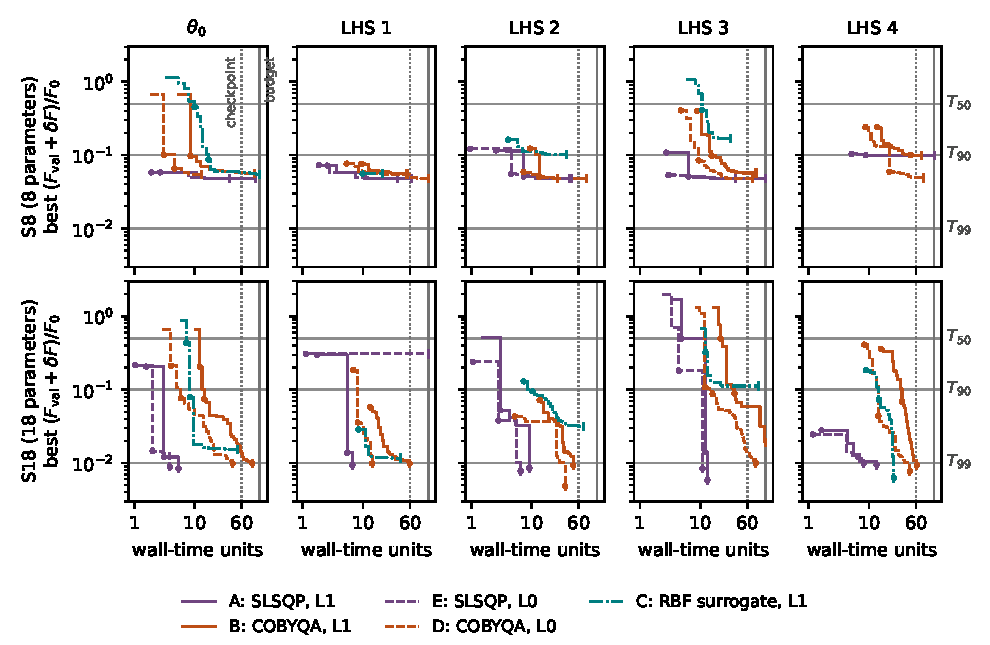
\includegraphics[width=.92\linewidth]{figures/exp2-quality.pdf}
\caption{How fast each method improves. Each panel is one start
($\theta_0$ or Latin-hypercube start LHS~1--4) in one space; each curve is
one method's best credited $(F_{\mathrm{val}}+\delta F)/F_0$ so far, that
is, its validated objective plus the allowance $\delta F$, against charged
wall time (repeat~1, log axes). Lower is better. The labelled grey lines are
the targets $T_{50}$, $T_{90}$ and $T_{99}$, and a dot marks a curve's
first crossing of each; the dotted and solid verticals are the 60-unit
checkpoint and the 120-unit budget. Each curve ends at the run's actual stop
(tick); a missing curve means the run had no credited validation.}
\label{fig:exp2-quality}
\end{figure}

\paragraph{Time to target.}
Figure~\ref{fig:exp2-time} gives the charged time to each target, per
start, and Table~\ref{tab:exp2-time} in Appendix~\ref{sec:exp2-times} lists
the values. In repeat~1, only three crossings occur
after the 60-unit checkpoint, all at $T_{99}$ in S18: two by B and one
by D.

Table~\ref{tab:exp2-ratios} (Appendix~\ref{sec:exp2-times}) gives paired time ratios. A ratio is formed
only when both methods attain the target from that start; no finite ratio
is derived from a censored cell. Wherever both reach a target from the
same start, gradient-based SLSQP gets there sooner than COBYQA at the same
coarse resolution. At L1 (B/A), the geometric-mean ratio is 3.10--3.25 in
S8 and 5.06--7.79 in S18. At L0 (D/E), it is 2.45--2.75 and
3.14--7.20.
All 45 finite optimizer-contrast pairs (by space, target and start) favor
SLSQP, with ratios from 1.46 to 21.5. The coarse mesh shortens the time by
a smaller factor: the geometric-mean E/A ratio is 0.62--0.79 and D/B is
0.45--0.56. Against D, the inexpensive derivative-free physical
competitor, A's lead in S8 comes mostly from validation: D needs more
validated incumbents before it crosses (a median of six against two), and
each costs a full validation. As charged, A is faster than D by a
geometric mean of 1.68--1.83 in S8; excluding the validation charges it is
1.15--1.16 (Appendix~\ref{sec:exp2-times}). In S18 A's lead is 2.25--4.32
as charged and 1.92--3.19 without validation. This contrast changes
both the optimizer and the resolution; one of its 25 pairs is a near tie
(0.99, S8 LHS~2 at $T_{90}$: D is 0.75\% faster, within the timing noise
between repeats).

\paragraph{Validation charges.}
Validating every new incumbent makes validation the largest single
charge (Table~\ref{tab:exp2-validation} in Appendix~\ref{sec:exp2-times}). One validation costs a median of
0.87 units over the 3,350 completed validations (range 0.55--1.10), and
validation takes 53\% of all charged time, 2--90\% per run. SLSQP crosses
a target after few validations, but most of its time to a target is
validation; COBYQA at L1 (B) needs more validations, which are a smaller
part of its time. Excluding the validation charges up to each crossing, the
same-resolution geometric means rise to 5.41--5.66 (B/A) and 5.55--5.56
(D/E) in S8, and to 8.84--13.58 and 7.92--15.27 in S18, so the
ratios as charged are conservative for the optimizer contrast. The coarse
mesh cuts the remaining time more, by geometric means of 0.19--0.27 (E/A)
and 0.20--0.23 (D/B), but it does not make validation cheaper, which is why
its overall saving is only 1.3--2.2 times.

The speed of E has a reliability cost. E never produces a credited
validation from S8 LHS~4. From S18 LHS~1 it reaches $T_{50}$ but
then stalls at $0.28F_0$, missing $T_{90}$ and $T_{99}$. In four
start--target cells, D reaches a target that E misses. A, by contrast,
reaches every target that any method reaches, from every start. C attains
$T_{99}$ only once in S18 and reaches $T_{90}$ from two of five
S8 starts.

\begin{figure}[t]\centering
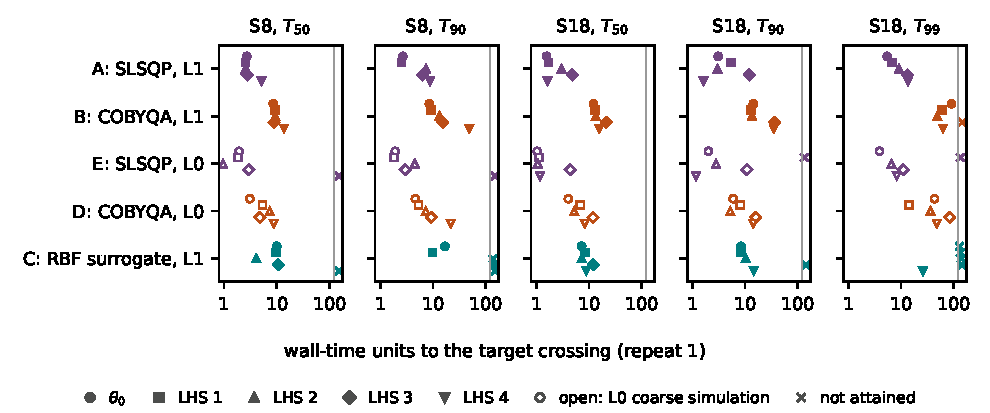
\includegraphics[width=.92\linewidth]{figures/exp2-time-to-target.pdf}
\caption{Charged wall time to each target crossing, repeat~1, for every
target attained by some run. Each row is a method, and each marker shape is
one start, offset vertically so that the same start can be followed across
methods. Filled markers: L1 coarse simulation; open markers: L0; crosses:
not attained within 120 units.}
\label{fig:exp2-time}
\end{figure}

\paragraph{Final refinement.}\label{sec:exp2-refinement}
The preregistered selection takes, for each method and space, the
lowest-$F_{\mathrm{val}}$ feasible design over both repeats, and the
earliest repeat-1 crossing of each attained target. With $\theta_0$ in
each space and identical designs merged, this gives 33 designs. Each
received the six registered checks: the primary L2 validation, L3, a
40-angle grid, Newton tolerance $10^{-12}$, an independently solved grid
shifted by $0.5^\circ$, and held-out currents $0.25$ and $0.75$. The 15
designs with zero stator offsets also received the conforming outer-band
Arkkio check on fresh meshes. All 213 checks completed
(Table~\ref{tab:exp2-refinement} in Appendix~\ref{sec:exp2-times}). These checks qualify the selected
designs only; they do not check each of the study's 111 repeat-1
target crossings.

The refinement used a hash-verified copy of the study outputs on a
different host (Appendix~\ref{sec:protocol-details}). Spatial refinement is the largest change. Over all 33 designs, L3 moves
$F$ by $-4.0\%$ to $+6.3\%$. Over the 25 target crossings alone, the range
is $-4.0\%$ to $+1.1\%$. The largest increase belongs to the overall best
design, D's in S18, whose $F$ rises from $0.0044F_0$ to $0.0047F_0$.
Angular and nonlinear effects are small: the 40-angle and shifted grids
change $F$ by at most $0.11\%$, and the tighter Newton tolerance by less
than $1.1\times10^{-5}$ relative. The conforming estimator gives $1.1\%$ to
$4.4\%$ more ripple than the order-93 coupling on the S8 designs, and
$2.0$--$2.1\%$ more at $\theta_0$. All 25 target crossings still satisfy
their target, allowance included, at L3; the smallest remaining margin is
1.2\% of the target. Every candidate also satisfies the full-current mean
floor in the primary, L3, 40-angle, tight and shifted checks, the closest
by 0.012\%. The refinement therefore confirms the selected crossings and
leaves the time-to-target comparison unchanged. At held-out currents
0.25 and 0.75, part of S18's extra reduction is lost
(Appendix~\ref{sec:exp2-times}).

\section{Post-hoc ablations: adjoint against finite-difference gradients}\label{sec:exp2-fd}
The contrast of Section~\ref{sec:optimization} changes the search strategy
and the gradient source together. Two ablations change only how SLSQP
obtains its gradient, and therefore what the gradient costs. Both were
added after the main outcomes were known and are not part of the
preregistered study; each public protocol was frozen before any of its
runs (Code and data availability).

\paragraph{Protocols.}
FD-cold is the safeguarded SLSQP of A with identical bounds, constraints,
restoration, validation policy, targets, mean floor and stopping rules.
Only the gradients of the objective and of the mean constraint change: they
are forward differences with a step of $10^{-6}$ in each coordinate's
physical unit (metres for the lengths and offsets), reusing the base value,
so one gradient costs $n$ extra coarse forwards, the stencil solves
($n=8$ in S8 and 18 in S18). Each stencil solve is an ordinary coarse
forward on the base point's mesh generation, and like every coarse
forward in the preregistered coarse configuration it starts Newton-cold
(all 40 traces record a cold start). A component whose forward step is
unusable (outside the box, unbuildable or on another mesh generation) takes
the backward step, as 8\% of components did; no gradient was refused.
FD-warm, the second arm, is FD-cold except that each stencil solve starts
Newton from its base point's retained converged state on the same mesh
generation, which makes it the stronger finite-difference competitor.
Every solve is charged, and the geometry-constraint Jacobians remain
analytic. Every run is one single-threaded process, so the $n$ stencil
solves run one after another and the time ratio is also a ratio of
compute; solving the stencil in parallel would shorten the wall time per
gradient but not its compute. Each arm runs with A rerun unchanged in the
same session (A$'$), sharing host, time unit and load, from the five starts
in both spaces on the L1 coarse simulation at 120 units: FD-cold with two
repeats (40 runs), FD-warm with repeat~1 only (20 runs), as its protocol
fixed in advance because FD-cold's repeats had agreed to about 1\% (a
median 1.0\% per primary crossing time) and the estimand uses repeat~1. The
primary estimand is, per start, the repeat-1 time ratio to the primary
target, $T_{90}$ in S8 and $T_{99}$ in S18; a censored cell gives no
finite ratio.

\paragraph{Results.}
Both finite-difference arms and both controls reach $T_{50}$ and $T_{90}$
in S8 and all three targets in S18 from all five starts; none
reaches $T_{99}$ in S8, and no cell is censored. Against the stronger
baseline, the adjoint reaches the primary target sooner from every start
(Fig.~\ref{fig:exp2b}): the geometric-mean FD-warm/A$'$ ratio is 1.71 in
S8 (range 1.68--1.77) and 2.70 in S18 (2.62--2.79). Against
cold-started stencils it is 2.47 (2.45--2.52) and 4.11 (3.84--4.33), with
repeat 2 giving 2.49 and 4.04 (Table~\ref{tab:exp2b-ratios}); compared
across sessions, FD-warm takes about 0.72 and 0.68 of FD-cold's time in seconds.
All three arms cross each primary target after the same number of
validations from every start, with one exception at a secondary target
(Appendix~\ref{sec:exp2-times}), so each gap is mainly the cost of the
gradient. Excluding the validation charges up to each crossing, FD-warm/A$'$
becomes 3.23 and 6.10, and FD-cold/A$'$ 5.58 and 10.07.

\begin{figure}[t]\centering
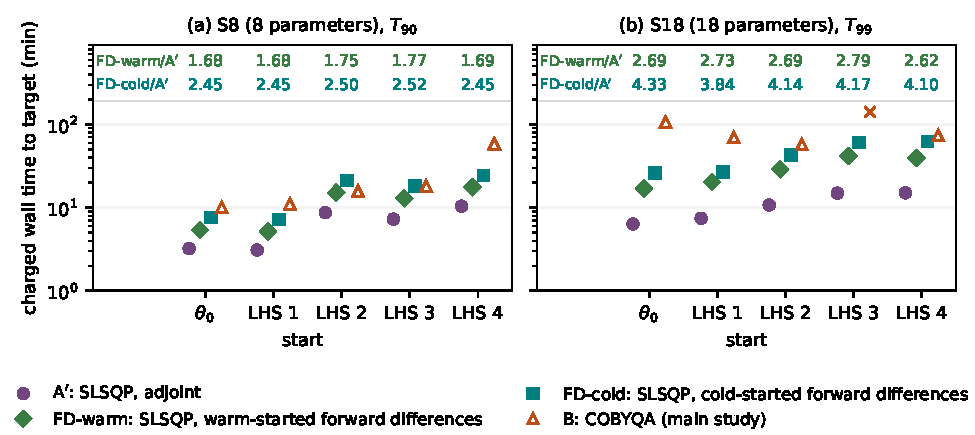
\includegraphics[width=.92\linewidth]{figures/exp2b-per-start.pdf}
\caption{Charged wall time, in minutes, to the primary target from each
start (repeat~1): A$'$ (SLSQP with adjoint gradients, from the FD-warm
session), FD-warm and FD-cold (the same SLSQP with warm- and cold-started
forward-difference gradients, from their own sessions), and B (COBYQA,
main study). Minutes avoid the 3--6\% differences between the sessions'
time units (1 unit is 1.11 to 1.18 minutes). The cross marks the start from
which B did not reach $T_{99}$; it is drawn at B's 120-unit budget. The two
labelled rows above the line give each start's FD-warm/A$'$ and
FD-cold/A$'$ ratio of charged time, each formed within its own session:
the FD-cold ratio divides by the A$'$ of the FD-cold session, which is not
the plotted A$'$ marker.}
\label{fig:exp2b}
\end{figure}

\paragraph{Gradient factor and optimizer factor.}
Against the main study, B/A $\approx$ (B/FD-warm)(FD-warm/A$'$) splits the
SLSQP-versus-COBYQA ratio into a gradient factor, finite-difference against
adjoint SLSQP, and an optimizer factor, COBYQA against finite-difference
SLSQP. Table~\ref{tab:decomp} gives both splits over the starts where B
attains the primary target (all five in S8; four in S18, where B misses
LHS~3). Of SLSQP's 3.10-fold (S8) and 7.79-fold (S18) advantage over
COBYQA, the gradient accounts for a factor of 1.71--2.47 and 2.68--4.10, and
the optimizer for 1.22--1.76 and 1.91--2.92. The lower gradient factor and
the higher optimizer factor belong to FD-warm, the cheaper finite-difference
baseline; which baseline applies elsewhere depends on whether a solver can
reuse the base point's state. COBYQA was slower than FD-warm from every
start, by as little as 1.01 at S8 LHS~2, whereas against FD-cold it matched
or beat SLSQP from two of five S8 starts (B/FD-cold 0.70 and 0.95). In
seconds, which removes the 3\% difference between the main and FD-warm
sessions' units, B/FD-warm is 1.81 and about 3.0 (per start in
Appendix~\ref{sec:exp2-times}).

\begin{table}[htbp]\centering\small
\caption{The gradient factor and the optimizer factor at the primary
targets: geometric means over the starts where B attains the target (five
in S8, four in S18), each ratio formed within one session's units. The
products close the main study's B/A only approximately, because their
factors come from different sessions.}
\label{tab:decomp}
\begin{tabular}{lrr}\toprule
 & S8, $T_{90}$ & S18, $T_{99}$\\\midrule
Total: COBYQA against adjoint SLSQP (B/A, main study) & 3.10 & 7.79\\
\addlinespace
\multicolumn{3}{l}{\emph{Against warm-started finite differences}}\\
\quad Gradient factor (FD-warm/A$'$) & 1.71 & 2.68\\
\quad Optimizer factor (B/FD-warm) & 1.76 & 2.92\\
\quad Product & 3.02 & 7.82\\
\addlinespace
\multicolumn{3}{l}{\emph{Against cold-started finite differences}}\\
\quad Gradient factor (FD-cold/A$'$) & 2.47 & 4.10\\
\quad Optimizer factor (B/FD-cold) & 1.22 & 1.91\\
\quad Product & 3.02 & 7.82\\
\bottomrule\end{tabular}

\end{table}

\paragraph{Where the time goes.}
Figure~\ref{fig:decomp} splits each arm's mean time to the primary target
into validation, the gradient and the rest (coarse forwards, mesh motion
and optimizer work). The three SLSQP arms spend nearly the same time on
validation and on the rest, because they cross after the same validated
designs: together 5.3--5.4 units in S8 and 8.0--8.1 in S18. The gradient is what
differs. A$'$'s adjoints take about 5\% of its time to the target, 0.30 and
0.51 units, against 4.37 and 14.91 units (45\% and 65\%) for FD-warm's
stencils and 8.72 and 27.47 units (62\% and 77\%) for FD-cold's. A free
gradient would therefore shorten A$'$'s time to the target by only 5--6\%:
the end-to-end ratios are bounded by the validation and coarse forwards
that every arm pays, not by the adjoint. This is why they fall well below
the per-gradient cost ratios of 18--70 below.

\begin{figure}[t]\centering
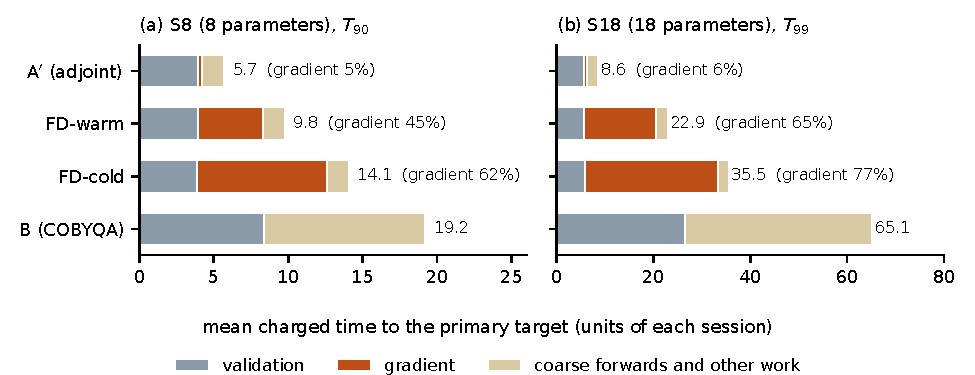
\includegraphics[width=.92\linewidth]{figures/decomp.pdf}
\caption{Mean charged time to the primary target, split into validation
(all validations up to and including the crossing), the gradient (FD-warm's
and FD-cold's stencil solves; A$'$'s adjoints, estimated as the number of
evaluations times the run's mean adjoint charge per evaluation) and the
rest, over the starts of Table~\ref{tab:decomp}. A$'$ is from the FD-warm
session; FD-cold's own A$'$ differs by less than 1\%. B has no gradient;
its rest includes its initial interpolation set. Each bar is in its own
session's unit; the bar labels give the total and, for the SLSQP
arms, the gradient's share of it.}
\label{fig:decomp}
\end{figure}

\paragraph{Gradient cost.}
Costs are in each session's unit, the median cold validation forward (66.66
and 69.09\,s). One adjoint gradient costs A$'$ 0.057 and 0.061 units with
eight and 18 parameters. One finite-difference gradient costs FD-cold 1.90 and
4.25 units, about 0.24 units per cold stencil solve, 33 and 70 times the
adjoint; it costs FD-warm 0.97 and 2.36 units, against 0.054 and 0.059 for
the adjoint in FD-warm's session, 18 and 40 times as much. A warm
stencil solve is charged about half a base coarse forward
(Appendix~\ref{sec:exp2-times}). Two factors shrink the per-gradient ratios. First, every coarse
evaluation costs a coarse forward that both arms pay. As a median over runs
of coarse-simulation time per coarse forward, it is 0.240 and 0.236 units for FD-cold
against 0.232 and 0.245 for its A$'$, and 0.220 and 0.238 for FD-warm's A$'$.
FD-warm's coarse-simulation time also contains its warm stencils, so for FD-warm we take
the median charge of one base coarse forward, 0.220 and 0.233 units (0.216
and 0.233 for its A$'$ on the same measure). An evaluation with a gradient
therefore costs FD-cold 7.4 and 14.7 times as much as A$'$. Second, A$'$
requests a gradient at every evaluation, whereas up to the primary
crossing FD-cold and FD-warm request one at a median 83.3\% of their evaluations
in S8 and at 76.9\% and 71.4\% in S18. With both factors the expected
ratios are 6.3 and 11.5 for FD-cold and 3.8 and 6.5 for FD-warm, against the
measured 5.58 and 10.07 and 3.23 and 6.10 once validation is excluded;
Appendix~\ref{sec:exp2-times} discusses the 6--16\% excess.

From 8 to 18 parameters ($n$ grows 2.25-fold) the per-gradient cost ratio
grows 2.2-fold against FD-warm and 2.1-fold against FD-cold, as a cost
proportional to $n$ predicts, but the end-to-end ratio grows only
1.6-fold (1.71 to 2.70) and 1.7-fold (2.47 to 4.11), because validation
and coarse forwards do not grow with $n$. The two spaces also differ in
primary target and in mesh-motion map; at the common target $T_{90}$,
FD-warm/A$'$ is 1.71 in S8 and 2.59 in S18, and FD-cold/A$'$ 2.47 and
3.86. Two spaces do not determine a rate, and we do not extrapolate.

\paragraph{Gradient accuracy.}
FD-cold's L1 gradients pass the max-norm check, and their one component-wise
failure is forward-difference truncation on a small component
(Appendix~\ref{sec:exp2-times}). At the frozen Newton tolerance, warm
stencils are less accurate: FD-warm's max-norm errors are 0.92 to 1.08
times FD-cold's, but its component-wise check fails at all four points, on
small components and once with a reversed sign, from an offset that the
warm stencil objectives share and that a central difference removes
(Appendix~\ref{sec:exp2-times}). The final checks of the selected
designs of all three arms keep every target crossing within its target at
L3, with at least 15\% margin (Appendix~\ref{sec:exp2-times}).

\section{Design-gradient verification}\label{sec:gradients}
\subsection{Differentiated model and excitation policy}
For a design vector $p$, the converged state $z$ contains the reduced
potential and, for harmonic coupling, its multipliers. Writing the full
constrained residual as $R(z,p)=0$, the discrete adjoint is
\begin{equation}
 R_z^T\psi=F_z^T,\qquad
 \frac{\dd F}{\dd p}=F_p-\psi^T R_p.
 \label{eq:adjoint}
\end{equation}
We differentiate mesh coordinates, element terms, magnet sources, current
loads, harmonic constraints and the torque functional. The explicit
coordinate derivative of Arkkio is included for conforming coupling.
Fixed-topology mesh motion $X(p)$ supplies the chain rule
$\dd F/\dd p_k=\langle\dd F/\dd X,\partial X/\partial p_k\rangle$
for geometric parameters, with direct terms added where needed.

The 12 parameters comprise nine geometric lengths (MAG, MH, MW,
SW1--SW4, SD1 and Sr1), axial length, operating angle and radial scale.
The two designs are the initial parameters and an interior point halfway
toward the saved optimized scalar parameters
(Appendix~\ref{sec:parameters}). This verifies a local scalar
parametrization. The reference's optimized geometry also uses grouped
surface-control displacements; reproducing its 12 scalar values alone
does not reproduce that geometry. The gradients that the optimizers of
Section~\ref{sec:optimization} used, including the grouped offsets of S18
and its mesh-motion map, are checked separately there.

The excitation rule changes these derivatives. Holding peak current fixed
differs from the reference optimizer's rule, which holds winding-group-1
current density fixed (Appendix~\ref{sec:cost} defines both). At L1
(harmonic coupling, coupling torque, full current), the mean-torque
derivative with respect to the stator tooth width SW1 is $+1.68$\,N\,m/m
under fixed current and $-220.85$\,N\,m/m under fixed group-1 density
(Fig.~\ref{fig:gradients}): a wider tooth narrows the slot and lowers
current under the density rule. At this state the policy changes seven of
the ten geometric/scale derivatives and reverses the mean-torque signs for
SW1, SW4 and SD1. The fixed-size problem of Section~\ref{sec:optimization}
holds physical current fixed for every method.

\subsection{Finite differences and Taylor remainders}
The derivative objectives are mean torque and population standard
deviation on the ten even mechanical angles, matching the reference's
optimization grid. Central differences move the same mesh at $p\pm h e_k$;
step sweeps separate truncation from floating-point and nonlinear-solve
error. We also check the first-order remainder
$|F(p+h e_k)-F(p)-h\,\dd F/\dd p_k|$ for quadratic decay.

Across initial and perturbed designs, L0--L2 and the recorded loaded
current/rule subsets, there are 800 objective--parameter records. They pool
harmonic/coupling-torque and conforming/Arkkio evaluations. The fixed-density
MAG, MH and MW records repeat 96 fixed-current comparisons byte-for-byte,
leaving 704 distinct comparisons. Of these, 688 have a best-step relative
error at most $2.8\times10^{-7}$; the maximum is $1.07\times10^{-5}$ for
a small Sr1 ripple derivative. This is a best-step verification statistic,
not the accuracy of a finite-difference step chosen in advance.
Figure~\ref{fig:gradients} includes the 704 distinct cases and an explicit
Taylor sweep. The artifact retains every step, rejected displacement and
relative error. The recorded subsets do not form a full factorial study.
Of 592 eligible distinct loaded comparisons, 530 have a quadratic
Taylor-remainder window spanning at least four decades of step size.
Verified is not the same as model-independent: at the same design the two
model--estimator pairs give ripple sensitivities whose box-scaled vectors
differ by 6.7\% and 10.2\% of their norm, more than either changes under
mesh refinement. Appendix~\ref{sec:cost} gives the Taylor windows, the
weaker zero-current checks, mesh convergence and this model dependence.

\begin{figure}[!htb]\centering
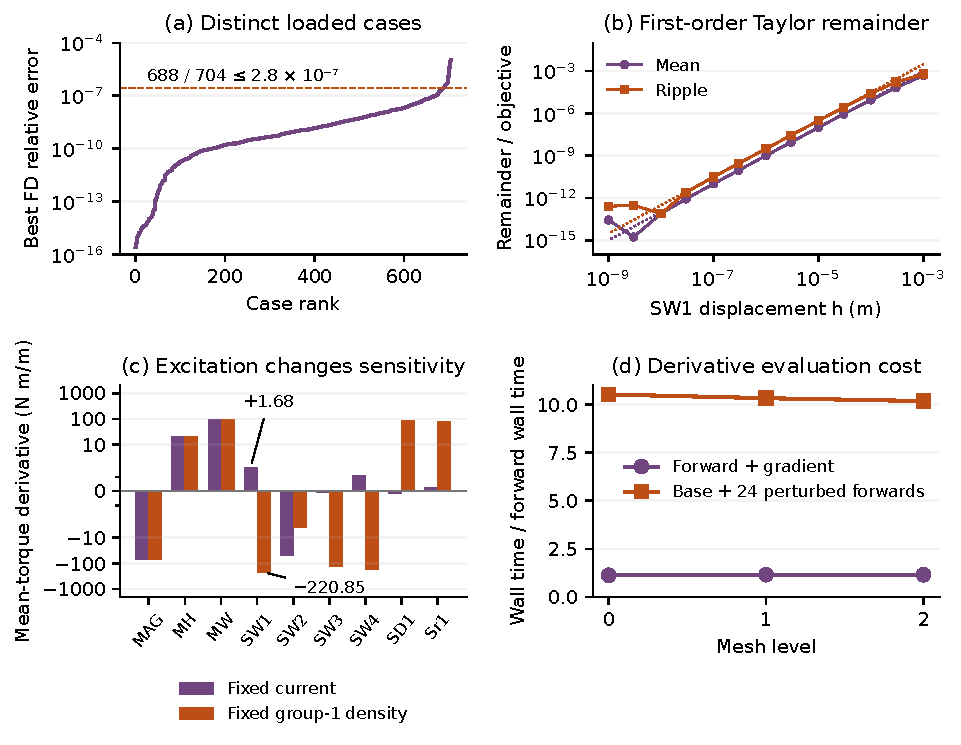
\includegraphics[width=.72\linewidth]{figures/design-gradients.pdf}
\caption{Discrete gradient evidence. (a) The 704 distinct loaded best-step
finite-difference errors, sorted, pooling harmonic/coupling-torque and
conforming/Arkkio objective--parameter cases. (b) SW1 Taylor remainders at L1, initial design,
full current, harmonic coupling and coupling torque, fixed current; the
plotted remainders are divided by $|F(p)|$, and dotted $h^2$ guides are anchored at $h=10^{-5}$\,m. (c) Mean-torque sensitivities for the nine geometric
parameters under two current rules at that same state; the vertical axis
is symmetric-log, linear within $\pm2$\,N\,m/m. (d) Recorded cost
ratios for harmonic coupling at tolerance $10^{-14}$; gradients include
the forward evaluation, and FD includes its shared base forward.
L0/L1 use medians of three runs, L2 a single run; the seconds are in
Appendix~\ref{sec:cost}.
These timing data were collected under uncontrolled host load.}
\label{fig:gradients}\end{figure}

On one loaded host, across L0--L2, both couplings and tolerances $10^{-8}$
and $10^{-14}$, the full gradient of both aggregate objectives with respect
to all 12 parameters costs 1.13--1.20 forwards, whereas central differences
cost 8.2--10.5 including the shared base solve (Fig.~\ref{fig:gradients}d;
Appendix~\ref{sec:cost} gives the protocol and seconds). A forward here is
one ten-angle sweep at full current on a multithreaded host, not the
60-solve, single-core forward of Section~\ref{sec:optimization}; the two
studies' cost ratios are not interchangeable.

\section{What transfers, and limits}\label{sec:discussion}
Three findings should transfer beyond this motor. First, SLSQP's advantage
over a derivative-free search factors into a gradient factor and an
optimizer factor, and both matter: here the gradient factor was 1.71--2.47
with eight parameters and 2.68--4.10 with 18, and the optimizer factor
1.22--1.76 and 1.91--2.92 (Table~\ref{tab:decomp}). Second, with the
optimization path held fixed, the gradient factor is a ratio of
end-to-end times, not of gradient costs. The adjoint made the gradient
about 5\% of the time to target, so the time every arm spends on
validation and coarse forwards bounds the factor; per-gradient cost
ratios of 18--70 became end-to-end ratios of 1.71--4.11, and from 8 to 18
parameters the per-gradient ratio grew about as $n$ while the end-to-end
ratio grew 1.6- to 1.7-fold. The factor also depends on how the stencil is
solved: warm-starting it halved the cost of a stencil solve and cut the
gradient factor from 2.47 and 4.11 to 1.71 and 2.70, at some cost in
accuracy on small components, and a cheaper gradient still, such as a
direct or semi-analytic sensitivity, would shift more of the advantage to
the optimizer factor. Third, validating each incumbent compresses
same-resolution ratios toward one and inflates SLSQP's lead over the
coarse competitor D, which needs more validated incumbents
(Section~\ref{sec:optimization}).

The evidence has clear limits. It is a paired case study over five
deterministic starts of one motor; the ratios are not population estimates.
The ablations are post hoc; FD-cold's forward differences carry a truncation
error and FD-warm's warm stencils a Newton-tolerance offset, each exceeding the
per-component check limit on small components (Section~\ref{sec:exp2-fd}). CMA-ES and other population or
multi-start methods remain untested.
Method C ran with the preregistered settings of
Appendix~\ref{sec:settings} and was not tuned; its low attainment bounds
this configuration, not radial-basis surrogates in general. No reduced
physical model, such as a nonlinear magnetic equivalent circuit
\citep{kemmetmueller2015}, a waveform-targeting surrogate \citep{roomi2022}
or an adaptive reduced model \citep{wen2023}, was compared: D searches a coarse finite-element simulation, not such a baseline, and
the slotless screening control of Appendix~\ref{sec:slotless} cautions
against inferring an advantage from parameter count alone. The forward model is two-dimensional and
magnetostatic, without thermal, demagnetization, fatigue, end-effect or
loss models, and is compared with published computational artifacts, not
with measurements on a physical motor.

Cheap, verified gradients also make methods affordable that this study did
not test. Second-order information is one: Hessian-vector products through a
second-order adjoint, or quasi-Newton methods driven by exact gradients beyond
the BFGS update inside SLSQP. Gradient-enhanced population and multistart
searches are another, such as particle swarms or CMA-style searches seeded or
steered by adjoint gradients, with runs in parallel across starts; every run
here used one single-threaded core. Each still pays for validation and coarse
forwards, which already bound the end-to-end gain (Fig.~\ref{fig:decomp}), and
can gain beyond that only by needing fewer of them or, in wall time but not in
compute, by running them in parallel. A natural next problem for the same
pipeline is the rotor flux-barrier design of synchronous reluctance machines,
a classic shape-optimization target because their torque ripple is high;
gradient-based free-form shape optimization has already been applied to such a
machine \citep{gangl2022multi}.

\section{Conclusion}
On a common validation simulation, SLSQP with adjoint gradients reached the
primary ripple targets 3.10 and 7.79 times sooner than COBYQA with 8 and 18
parameters, and post-hoc ablations split that advantage into two factors.
The gradient factor, adjoint against forward differences in the same
SLSQP, was 1.71 and 2.70 against warm-started stencils and 2.47 and 4.11
against cold ones; the optimizer factor, COBYQA against finite-difference
SLSQP, made up the rest. The adjoint left the gradient about 5\% of the
time to target, so validation and coarse forwards now bound the
remaining gain. Before trusting such a gradient, check what it
differentiates: interface order and excitation rule change the objective
or its sensitivities.

\section*{Author contributions}
C.D. wrote the four-layer operator specification that GEODE realizes
\citep{dunnavant2026whiteroom}, whose layers are unrelated to the mesh
levels L0--L3, and gave design input and review. R.W. ran the work and the
software agents that carried it out and is responsible for the results.

\section*{Code and data availability}
The original forward and gradient evidence is fixed at GEODE commit
\href{https://github.com/rjwalters/geode-fem/tree/910593bad6f64f9f01671c2632b57034e72b9c61}{\texttt{910593ba}}.
The repository contains the
\href{https://github.com/rjwalters/geode-fem/tree/910593bad6f64f9f01671c2632b57034e72b9c61/benchmarks/motor_reference/forward_harmonic}{raw motor runs and analysis},
\href{https://github.com/rjwalters/geode-fem/tree/910593bad6f64f9f01671c2632b57034e72b9c61/benchmarks/motor_reference/geometry}{geometry and mesh-generation scripts},
\href{https://github.com/rjwalters/geode-fem/tree/910593bad6f64f9f01671c2632b57034e72b9c61/benchmarks/motor_shape_gradient/design}{design-gradient sweeps and timing records},
and \href{https://github.com/rjwalters/geode-fem/tree/910593bad6f64f9f01671c2632b57034e72b9c61/benchmarks/motor_nonlinear_m1}{solver verification logs}.
Candidate-validation records are pinned at
\href{https://github.com/rjwalters/geode-fem/tree/224332c526be1191183af82b610973c7778de720/benchmarks/motor_validation}{\texttt{224332c5}},
and independent reference reruns at
\href{https://github.com/rjwalters/geode-fem/tree/8acd21ecf85d89fe077275a3c04ca70b53963d43/benchmarks/motor_reference/reference_refinement}{\texttt{8acd21ec}}.
Reference data are extracted from the authors'
\href{https://github.com/MichaelWiesheu/ICEMsnapshot/tree/b145aaf4ab1a6424828bc941eaf172f48fa0d458}{ICEM snapshot at \texttt{b145aaf4}},
a later repository revision rather than a claim to the original conference
release. Source hashes, extraction checks and the upstream GPL-3.0-or-later license
are retained. Recomputing the physical study requires the separately
documented mesh and solver commands; the benchmark READMEs record the
GEODE-side Gmsh and Rust toolchain versions.

\begin{sloppypar}
The matched optimization study (Section~\ref{sec:optimization}) follows the
optimization harness at
\href{https://github.com/rjwalters/geode-fem/tree/9486a9da58beeca91968d4d3608f06b998abff45/benchmarks/motor_optimization}{\texttt{9486a9da}},
the source of the study's evaluator, and its
\href{https://github.com/rjwalters/geode-fem/tree/9486a9da58beeca91968d4d3608f06b998abff45/benchmarks/motor_optimization/runs}{coarse-gradient finite-difference records};
the final-refinement binary was built from the program at
\href{https://github.com/rjwalters/geode-fem/blob/63b3e3d8bbc30504f845eebb5b78e8be6a2ee12f/crates/geode-core/examples/icem_final_refinement.rs}{\texttt{63b3e3d8}},
which differs from the version at
\href{https://github.com/rjwalters/geode-fem/blob/3e4ee0c63a86dbf014a76c9faf04dd962da16911/crates/geode-core/examples/icem_final_refinement.rs}{\texttt{3e4ee0c6}}
only by one unused import.
This paper's PDF and \LaTeX{} source are archived at
\href{https://doi.org/10.5281/zenodo.23580548}{doi:10.5281/zenodo.23580548}.
The paper package is the directory
\href{https://github.com/rjwalters/geode-fem/tree/main/papers/motor-gradient-optimization/motor-gradient-optimization.21}{\texttt{papers/}\allowbreak\texttt{motor-gradient-optimization/}\allowbreak\texttt{motor-gradient-optimization.21}}
of the \href{https://github.com/rjwalters/geode-fem}{GEODE repository}. It
contains a manifest of every copied input with its source commit and
SHA-256, the figure inputs and regeneration scripts (rebuilding the figures
does not require rerunning FEM), four standard-library verifiers (one
entry point that runs the other three) that recompute the reported numbers
from those inputs, the per-run validation
histories and ledger charges, the 213 final-check results, copies of the
coarse-gradient checks, and the study's SHA-256 inventory of all 5,453
output files. The inventory was taken when the session finished; its
existence by 2026-10-20 03:50~UTC is timestamped (RFC~3161 and
OpenTimestamps), and each extracted run and session record is bound to it
by hash. The session, calibration and anchor-recomputation records are
included, as is an export of the governing preregistration comments taken
on 2026-10-18 at 09:34~UTC, before the main session began at 18:16~UTC.
\end{sloppypar}

For the two post-hoc ablations (named \texttt{F} and \texttt{F\_w} in their records), the package holds the 40 and 20 run
extracts with their evaluation timelines, the setup records, each session's SHA-256 inventory (2,118 and
1,180 files) with its RFC~3161 and OpenTimestamps records, the final-check
results, the comparison of the original and rebuilt refinement binaries,
and an export of each protocol. FD-cold's evaluator source is
\href{https://github.com/rjwalters/geode-fem/tree/5cc86ad81aeea4847a2608fcafde22a1bbfb6990/benchmarks/motor_optimization}{\texttt{5cc86ad8}},
its L1 gradient check is pinned at
\href{https://github.com/rjwalters/geode-fem/tree/74843242db03e8d57edf971420171064bf19f107/benchmarks/motor_optimization/harness}{\texttt{74843242}}
and its step sweep at
\href{https://github.com/rjwalters/geode-fem/tree/f94acad3f312c7d417830ff82b66a78a1ea89fb2/benchmarks/motor_optimization/harness}{\texttt{f94acad3}};
FD-warm's evaluator source and L1 checks are at
\href{https://github.com/rjwalters/geode-fem/tree/669029c5653cb5fe4724ec0c7525ba60c770975e/benchmarks/motor_optimization}{\texttt{669029c5}}.
FD-cold's \href{https://github.com/rjwalters/geode-fem/issues/1218}{protocol}
was posted at 22:34~UTC on 2026-10-20 and frozen by a comment at
23:00~UTC, before the first FD-cold run began at 02:07~UTC on 2026-10-21;
FD-warm's timeline is in Appendix~\ref{sec:exp2-times}. These are GitHub
timestamps, and neither protocol text was ever edited. The raw traces of all
three sessions, the 5,453, 2,118 and 1,180 inventory-listed files with the
inventories and their timestamp records, are packed in one archive with
each session's final-check requests and results, the ablations' selection
outputs and the binary comparison with the rebuilt binary:
\texttt{motor-paper-raw-traces.tar.zst} (2,790,582,024 bytes, SHA-256
\texttt{1dfbf3883a9f1f3d8ddc44f67ce594b8}\allowbreak\texttt{8291ec235a154337d24efa07a1b98b07}), deposited at
DOI \href{https://doi.org/10.5281/zenodo.23580550}{10.5281/zenodo.23580550}. Every file was checked against its inventory
when the archive was built, and the archive's manifest lists the SHA-256
of every file it holds. Given the unpacked archive, the package's verifiers
re-derive the run, timeline and final-check extracts of all three sessions
from the raw traces and results.

\appendix
\section{Field model details}\label{sec:fieldmodel}
\subsection{Nonlinear field equation}
The two-dimensional magnetic vector potential $A=A_z$ determines the
flux density $\mathbf B=(\partial_y A,-\partial_x A)$. Iron is described
by an isotropic reluctivity $\nu(|\mathbf B|^2)$, where reluctivity is
the inverse of permeability. For a test function $v$ that satisfies the
homogeneous constraints, the weak equation is
\begin{equation}
 \int_\Omega \nu(|\nabla A|^2)\nabla A\cdot\nabla v\dd\Omega
 =\int_\Omega J_z v\dd\Omega
  +\int_{\Omega_m}\mathbf M\cdot(\partial_y v,-\partial_x v)\dd\Omega.
 \label{eq:weak}
\end{equation}
Here $\mathbf M$ denotes the permanent-magnet source in
$\mathbf H=\nu\mathbf B-\mathbf M$. In the magnet,
$\mu_r=1.05$ and $B_r=1.4$\,T, so its source magnitude is
$H_c=B_r/(\mu_0\mu_r)$, not $B_r/\mu_0$. Its direction is $\pi/2$
in the rotor frame and rotates with the rotor. Air and windings have
$\mu_r=1$. The inner and outer circular boundaries have $A=0$.

We use continuous piecewise-linear triangles. With nodal vector $u$,
element gradients $g_i=\nabla\varphi_i$, $G=\nabla A$ and $s=G\cdot G$,
the residual derivative on one element is
\begin{equation}
 K^e_{ij}=|\Omega_e|\left[\nu(s)g_i\cdot g_j
       +2\nu'(s)(g_i\cdot G)(g_j\cdot G)\right].
 \label{eq:tangent}
\end{equation}
The second term is required when the material changes with field strength.
Newton steps use this consistent tangent, with damping and a stopping
reference independent of the initial guess. Constant potential offsets,
where allowed by the boundary conditions, do not change that reference.
The solver reports whether it stopped at the requested tolerance or an
estimated floating-point floor. All 500 baseline and sensitivity solves, and all 1,140
additional harmonic-coupling solves, stopped at the requested tolerance.

The iron law uses 47 tabulated M27 $B$--$H$ points from 0 to 2.30\,T.
Monotonicity is imposed on $H(B)$, not on $\nu(B^2)=H(B)/B$.
The tabulated $H/B$ is non-monotone up to about 0.75\,T.
The two material tangent eigenvalues must satisfy
\begin{equation}
 \nu>0,\qquad \nu+2s\nu'=\frac{\dd H}{\dd B}>0.
\end{equation}
The GEODE and reference interpolants agree to round-off between 0.05 and
2.25\,T. GEODE uses an odd cubic near zero and a continuous slope into the
vacuum-slope tail above 2.30\,T. The reference uses a low-field clamp and
a different last-knot slope. The maximum relative difference in
reluctivity near zero is 6.66\%; the last segment differs in $H$ by at
most $2.17\times10^{-4}$ relatively. Appendix~\ref{sec:controls} tests the
torque effect of the low-field difference.

\subsection{Rotation, coupling and torque}
At the modeled angles, the two circular traces have matching nodes after
rotation. Our conforming interface identifies their potentials, including
the antiperiodic sign on sector wrap-around. Writing the full nodal vector
as $u=P\hat u+u_D$, the reduced residual and tangent are
$\hat R=P^T R(P\hat u+u_D)$ and $\hat K=P^T K P$.
The rotor geometry and magnet source rotate together; currents use the
same mechanical angle in Eq.~\eqref{eq:current}.

We average Maxwell stress over the air gap using the Arkkio expression
\citep{arkkio1987}
\begin{equation}
 T(\beta)=\frac{L}{\mu_0(r_2-r_1)}
  \int_{\Omega_{\rm gap}}r B_r B_\theta\dd\Omega,
 \qquad(r_1,r_2)=(44,45)\ {\rm mm}.
 \label{eq:torque}
\end{equation}
Positive torque acts counter-clockwise on the rotor. All torques in this
paper include axial length and refer to the modeled sector. We apply no
factor of six when comparing with the saved reference arrays, despite a
per-length label appearing in the reference evaluation plots.

The alternative harmonic model imposes
\begin{equation}
 \int_{\Gamma_c}(A_s-A_r)e_n\dd\Gamma=0,\qquad
 e_n\in\{\sin(n\theta),\cos(n\theta)\},\quad n=3,9,\ldots,N_h,
\end{equation}
with maximum order $N_h=45$ unless stated otherwise. The 16 order-45
constraints match the reference's eight orders. Rotor and stator
retain distinct trace unknowns. With constraint matrix $C$, Lagrange
multipliers $\eta$ and reduced potential $\hat u$, Newton's method uses
the saddle tangent
\begin{equation}
 \begin{bmatrix}K&C\\ C^T&0\end{bmatrix}.
\end{equation}
The trace moments use the exact Fourier integrals of the piecewise-linear
hats. Rotation enters their centers; the constrained energy derivative gives
\begin{equation}
 T_c=-L\eta^T\frac{\partial(C^T\hat u)}{\partial\beta},
 \label{eq:couplingtorque}
\end{equation}
with the state held fixed in the partial derivative, consistent with
\citet{egger2022torque}. Forward comparisons use Arkkio for both GEODE
couplings to isolate the interface change; coupling torque is a separate
check. The derivative study uses coupling torque for the harmonic model
and Arkkio for the conforming model. The two objectives and their gradients
are consequently comparisons of those specified model--estimator pairs.
The optimization study's coarse simulation uses order-45 coupling torque and
its validation simulation order 93.

The main harmonic runs retain antiperiodic trace-end pairing. An additional
set frees those ends, matching the reference's treatment. The full-order
identity check is summarized in Section~\ref{sec:model}.

\subsection{Implementation checks}
The nonlinear implementation is checked against linear assembly, residual
finite differences, a manufactured solution and a saturated annulus with
an independent radial field relation. Sector tests compare the
constrained solution with a full-machine solve, check the reduced tangent
by finite differences, and exercise positive, negative and wrapped rotation
steps. Clockwise and counter-clockwise triangle orderings give equivalent
magnet sources and fields. The motor regression also detects changes in
magnet strength, magnet direction, phase ordering and rotation direction.
The verification records are linked in the data-availability section.

\section{Optimizer and search settings}\label{sec:settings}
Table~\ref{tab:settings} lists the settings a replication needs beyond
Section~\ref{sec:optimization}; the pinned harness documents them in full.
All methods work in the unit box $u\in[0,1]^n$ of the free coordinates,
minimize $F_r/F_r(\theta_0)$ on their coarse simulation $r$ and impose the
mean floor as $\mu_{r,1}/\mu_{r,1}(\theta_0)-1.0025\geq0$.
No method validates its start point, and a point validated once is not
validated again.

\begin{table}[H]\centering\small
\caption{Optimizer settings. $n$ is the number of free coordinates (8 or
18), $x_v$ the last admissible evaluated point and $x$ a refused request.}
\label{tab:settings}
\begin{tabular}{>{\raggedright\arraybackslash}p{.11\linewidth}>{\raggedright\arraybackslash}p{.83\linewidth}}\toprule
Method & Settings\\\midrule
A, E & SciPy SLSQP, \texttt{ftol} $10^{-15}$, \texttt{maxiter} $10^5$. Adjoint gradients of the objective and the mean constraint; analytic Jacobians of the geometry constraints. Safeguard: a refused request (unbuildable, mesh-infeasible or derivative undefined) aborts the current solve; the first admissible point $y_k=x_v+2^{-k}(x-x_v)$, $k=1,\ldots,20$, is restored and SLSQP restarts from it with fresh state, at most 20 times. Validation: each iterate the SLSQP callback reports.\\
B, D & SciPy COBYQA, $2n+1$ initial interpolation points, trust radius $0.1$ to $10^{-6}$, \texttt{maxiter} $=$ \texttt{maxfev} $=10^9$. A refused point returns NaN for objective and mean constraint; geometry constraints keep their values. Validation: the callback's best point whenever it changes, after the initial set.\\
C & Four cubic radial-basis interpolants, $\phi(r)=r^3$ with a linear tail: the three objective-current standard deviations, each over $\sqrt{F_r(\theta_0)}$, and the full-current mean, refitted after every evaluation. Initial design: the start and $u_0\pm\Delta_0e_i$, $\Delta_0=0.1$ ($n+1$ points). Subproblem: SLSQP on the surrogate in the box and $\|u-u_k\|_\infty\leq\Delta$, at most 200 iterations. Acceptance: a candidate better than the incumbent, feasible first (lower violation, then lower $F$). On acceptance with $\rho\geq0.75$ and a step of at least $0.9\Delta$, $\Delta\leftarrow\min(2\Delta,0.5)$; on rejection $\Delta\leftarrow\Delta/2$, with a geometry point $u_k\pm\Delta e_j$ after every second rejection. Stop at $\Delta<10^{-6}$. Refused points are skipped and count as rejections. Validation: each acceptance.\\
\bottomrule\end{tabular}
\end{table}

The Latin-hypercube starts \citep{mckay1979comparison} use seeds 1--4;
the computations use NumPy \citep{harris2020array} and SciPy
\citep{virtanen2020scipy}.

\section{Study protocol details}\label{sec:protocol-details}
\paragraph{Coarse gradients.}
Section~\ref{sec:gradients} verifies a different, scalar parameter set; the
gradients that A and E use were checked separately. In both spaces, the L1
coarse objective $F$ and full-current mean were compared with central
differences at $\theta_0$ and at an interior point, along a fixed
box-scaled direction and for three (S8) or four (S18) components,
including the offsets CPR1 and CPS1. With Newton tolerance $10^{-12}$, the
directional relative errors at $h=10^{-4}$ are $1.5\times10^{-8}$ to
$2.8\times10^{-7}$ for $F$ and $2.4\times10^{-9}$ to $4.7\times10^{-9}$ for
the mean, and the component errors at $h=10^{-6}$ are at most
$2.8\times10^{-6}$. The directional error falls by 72 to 156 times from
$h=10^{-3}$ to $10^{-4}$, as truncation error should. The evaluator's own
gradient replies at the coarse simulation's Newton tolerance of $10^{-8}$ agree at
the interior point within $3.1\times10^{-6}$ directionally; the largest
component error, $4.3\times10^{-5}$, belongs to the small Sr1 derivative.
At $\theta_0$, S18's offsets sit on their bounds, so the central
stencils there step outside the design box. The records are pinned with the
optimization harness (Code and data availability).

\paragraph{Session.}
The session ran on one AWS c7a.4xlarge host (x86-64; NumPy 2.5.4 and
SciPy 1.18.1 with OpenBLAS) with 15 concurrent single-threaded processes.
Before calibration, the host recomputed the initial-design validation
waveforms in both spaces. $F_0$ agreed with the canonical anchor to
$2.4\times10^{-13}$ relative, within the preregistered $10^{-9}$ tolerance,
and the two spaces agreed bit for bit. The calibrated unit was
$70.94\,\mathrm{s}$, the median of 45 concurrent cold validations. All 100
runs completed in one session with no recovery, deferral or contamination:
the one-minute load average peaked at 21.1, below the contamination
threshold of $1.5N=22.5$. The in-run cost totals 109~CPU-hours. Of the
100 runs, 38 stopped on reaching $T_{99}$, 46 on optimizer convergence and
13 at the budget. The other three are SLSQP runs (A) in S8 whose
solver stopped without converging: both repeats from LHS~2, after about 43
units, and repeat~1 from LHS~3, after 119 units.

\paragraph{Refinement host.}
The registered pipeline begins by capturing the closed study on its
original host, a step that could not be completed after that host had been
restarted. The refinement instead used a copy of the study outputs whose
integrity is established by a SHA-256 inventory of every output file, taken
when the session finished, and independently timestamped; the timestamps
establish that the inventory existed by 2026-10-20 03:50~UTC. It ran on a different host (Apple M3 Ultra,
macOS arm64). For the 16 selected designs validated on the moved reference
mesh, the primary check reproduces the study's $F_{\mathrm{val}}$ to below
$2.2\times10^{-12}$ relative. The other 15 candidates needed a fresh mesh,
which Gmsh triangulates differently on the two platforms; their $F$
differs by at most $1.7\times10^{-3}$ relative. The remaining two designs
are $\theta_0$ in each space, which reproduces $F_0$. The fresh-mesh
differences measure the sensitivity of $F$ to remeshing and are far below
the 10\% allowance $\delta F$.


\section{Per-start times, ratios and final checks}\label{sec:exp2-times}
\begin{table}[H]\centering\small
\caption{Charged wall-time units to the first attaining validation,
repeat~1. A dash means the target was not attained within 120 units.
$T_{99}$ was attained by no run in S8.}
\label{tab:exp2-time}\begin{tabular}{llrrrrr}\toprule
Space, target & Method & $\theta_0$ & LHS 1 & LHS 2 & LHS 3 & LHS 4\\\midrule
S8, $T_{50}$ & A & 2.7 & 2.5 & 2.6 & 2.7 & 5.1\\
 & B & 8.5 & 9.3 & 9.3 & 8.9 & 13.7\\
 & E & 1.9 & 1.8 & 1.0 & 3.0 & ---\\
 & D & 3.1 & 5.3 & 7.3 & 4.8 & 8.8\\
 & C & 10.0 & 9.8 & 4.1 & 10.6 & ---\\
\addlinespace
S8, $T_{90}$ & A & 2.7 & 2.5 & 7.4 & 6.4 & 8.8\\
 & B & 8.5 & 9.3 & 13.3 & 15.4 & 49.3\\
 & E & 1.9 & 1.8 & 4.5 & 3.0 & ---\\
 & D & 4.6 & 5.3 & 7.3 & 9.4 & 21.9\\
 & C & 16.9 & 9.8 & --- & --- & ---\\
\addlinespace
S18, $T_{50}$ & A & 1.6 & 1.7 & 3.0 & 4.8 & 1.6\\
 & B & 12.2 & 13.1 & 13.5 & 21.5 & 15.7\\
 & E & 1.0 & 1.1 & 1.1 & 4.4 & 1.2\\
 & D & 4.1 & 6.9 & 5.2 & 11.9 & 8.4\\
 & C & 7.3 & 8.4 & 7.3 & 12.1 & 8.9\\
\addlinespace
S18, $T_{90}$ & A & 3.1 & 5.4 & 3.0 & 12.0 & 1.6\\
 & B & 14.4 & 13.1 & 13.5 & 36.6 & 35.3\\
 & E & 2.0 & --- & 2.8 & 10.9 & 1.2\\
 & D & 5.9 & 8.1 & 5.2 & 15.9 & 14.3\\
 & C & 8.4 & 8.4 & 10.3 & --- & 14.6\\
\addlinespace
S18, $T_{99}$ & A & 5.4 & 6.6 & 9.1 & 13.1 & 13.4\\
 & B & 90.4 & 59.1 & 48.6 & --- & 62.3\\
 & E & 3.9 & --- & 6.5 & 10.9 & 8.3\\
 & D & 43.0 & 14.1 & 36.0 & 83.3 & 47.8\\
 & C & --- & --- & --- & --- & 25.9\\
\bottomrule\end{tabular}

\end{table}

\begin{table}[H]\centering\small
\caption{Paired per-start time ratios (repeat~1). B/A and D/E vary the
optimizer at fixed resolution; E/A and D/B vary the resolution; D/A
compares A with the coarse derivative-free competitor. Ratios above one
favor the denominator. Geometric means use the finite pairs only, so the
D/E and E/A means omit the starts where E failed to attain the target.}
\label{tab:exp2-ratios}\begin{tabular}{llrrl}\toprule
Space, target & Ratio & Finite pairs & Geometric mean & Per-start ratios\\\midrule
S8, $T_{50}$ & B/A & 5 & 3.25 & 3.18, 3.66, 3.63, 3.25, 2.66\\
 & D/E & 4 & 2.75 & 1.60, 2.90, 7.68, 1.61, ---\\
 & E/A & 4 & 0.68 & 0.72, 0.72, 0.37, 1.09, ---\\
 & D/B & 5 & 0.56 & 0.36, 0.57, 0.78, 0.54, 0.64\\
 & D/A & 5 & 1.83 & 1.15, 2.09, 2.85, 1.75, 1.71\\
\addlinespace
S8, $T_{90}$ & B/A & 5 & 3.10 & 3.18, 3.66, 1.80, 2.43, 5.61\\
 & D/E & 4 & 2.45 & 2.41, 2.90, 1.61, 3.17, ---\\
 & E/A & 4 & 0.62 & 0.72, 0.72, 0.61, 0.47, ---\\
 & D/B & 5 & 0.54 & 0.54, 0.57, 0.55, 0.61, 0.44\\
 & D/A & 5 & 1.68 & 1.72, 2.09, 0.99, 1.48, 2.49\\
\addlinespace
S18, $T_{50}$ & B/A & 5 & 6.49 & 7.76, 7.70, 4.51, 4.46, 9.59\\
 & D/E & 5 & 4.69 & 3.90, 6.14, 4.93, 2.72, 7.09\\
 & E/A & 5 & 0.63 & 0.66, 0.66, 0.35, 0.91, 0.72\\
 & D/B & 5 & 0.46 & 0.33, 0.52, 0.39, 0.56, 0.53\\
 & D/A & 5 & 2.97 & 2.58, 4.04, 1.75, 2.48, 5.09\\
\addlinespace
S18, $T_{90}$ & B/A & 5 & 5.06 & 4.64, 2.41, 4.51, 3.05, 21.54\\
 & D/E & 4 & 3.14 & 2.94, ---, 1.86, 1.46, 12.17\\
 & E/A & 4 & 0.79 & 0.65, ---, 0.94, 0.91, 0.72\\
 & D/B & 5 & 0.45 & 0.41, 0.62, 0.39, 0.44, 0.41\\
 & D/A & 5 & 2.25 & 1.91, 1.50, 1.75, 1.33, 8.74\\
\addlinespace
S18, $T_{99}$ & B/A & 4 & 7.79 & 16.65, 8.92, 5.33, ---, 4.65\\
 & D/E & 4 & 7.20 & 11.05, ---, 5.50, 7.65, 5.79\\
 & E/A & 4 & 0.72 & 0.72, ---, 0.72, 0.83, 0.61\\
 & D/B & 4 & 0.50 & 0.48, 0.24, 0.74, ---, 0.77\\
 & D/A & 5 & 4.32 & 7.91, 2.12, 3.94, 6.36, 3.56\\
\bottomrule\end{tabular}

\end{table}

\begin{table}[H]\centering\scriptsize
\caption{Final checks of the selected designs. ``best'' marks a method's
representative; ``A $T_{90}$'' marks the earliest repeat-1 crossing of that
target by that method. The L2 column is the primary check on the
refinement host. L3 and conforming changes are in percent; the 40-angle,
tight and shifted changes are relative, in units of $10^{-4}$. ``held-out'' is the objective at currents $0.25$ and
$0.75$ relative to $\theta_0$'s at the same currents. A dash means the
conforming check does not apply because stator offsets are nonzero.}
\label{tab:exp2-refinement}\begin{tabular}{lrrrrrrr}\toprule
Design & $F_{\mathrm{L2}}/F_0$ & L3 & g40 & tight & shifted & conf. & held-out\\
 & & (\%) & ($10^{-4}$) & ($10^{-4}$) & ($10^{-4}$) & (\%) & \\\midrule
\multicolumn{8}{l}{\emph{S8}}\\
$\theta_0$ & 1.0000 & $-1.3$ & $0.0$ & $0.0$ & $+0.1$ & $+2.1$ & 1.0000\\
best A & 0.0432 & $-0.4$ & $0.0$ & $0.0$ & $+0.1$ & $+4.4$ & 0.0472\\
best B & 0.0432 & $-0.5$ & $0.0$ & $0.0$ & $0.0$ & $+4.4$ & 0.0472\\
best C & 0.0489 & $-0.7$ & $+0.2$ & $0.0$ & $+0.5$ & $+4.1$ & 0.0524\\
best D & 0.0432 & $-0.5$ & $0.0$ & $0.0$ & $0.0$ & $+4.4$ & 0.0472\\
best E & 0.0434 & $-0.6$ & $+0.4$ & $0.0$ & $+0.9$ & $+4.4$ & 0.0473\\
A $T_{50}$, A $T_{90}$ & 0.0653 & $-2.9$ & $+0.7$ & $0.0$ & $+1.5$ & $+1.1$ & 0.0686\\
B $T_{50}$, B $T_{90}$ & 0.0881 & $-2.3$ & $+1.3$ & $0.0$ & $+2.6$ & $+3.2$ & 0.0866\\
C $T_{50}$ & 0.1472 & $-4.0$ & $+0.6$ & $0.0$ & $+1.3$ & $+3.3$ & 0.1508\\
C $T_{90}$ & 0.0507 & $-0.9$ & $+0.2$ & $0.0$ & $+0.5$ & $+4.0$ & 0.0543\\
D $T_{50}$ & 0.0920 & $-2.2$ & $+1.5$ & $0.0$ & $+3.0$ & $+3.3$ & 0.0899\\
D $T_{90}$ & 0.0594 & $-2.3$ & $+1.3$ & $0.0$ & $+2.6$ & $+1.6$ & 0.0609\\
E $T_{50}$ & 0.1105 & $-2.0$ & $+0.6$ & $0.0$ & $+1.1$ & $+1.2$ & 0.1104\\
E $T_{90}$ & 0.0660 & $-2.9$ & $+0.7$ & $0.0$ & $+1.5$ & $+1.1$ & 0.0694\\
\multicolumn{8}{l}{\emph{S18}}\\
$\theta_0$ & 1.0000 & $-1.3$ & $0.0$ & $0.0$ & $+0.1$ & $+2.0$ & 1.0000\\
best A & 0.0053 & $+2.6$ & $+0.4$ & $+0.1$ & $+0.5$ & --- & 0.0066\\
best B, B $T_{99}$ & 0.0085 & $-3.0$ & $-0.4$ & $0.0$ & $-1.2$ & --- & 0.0076\\
best C, C $T_{99}$ & 0.0057 & $-3.7$ & $+2.5$ & $0.0$ & $+5.0$ & --- & 0.0074\\
best D & 0.0044 & $+6.3$ & $+2.6$ & $+0.1$ & $+4.9$ & --- & 0.0076\\
best E & 0.0071 & $+2.6$ & $-1.5$ & $0.0$ & $-3.1$ & --- & 0.0087\\
A $T_{50}$ & 0.1874 & $+0.9$ & $-0.3$ & $0.0$ & $-0.6$ & --- & 0.1538\\
A $T_{90}$ & 0.0255 & $+1.1$ & $-0.1$ & $0.0$ & $-0.2$ & --- & 0.0248\\
A $T_{99}$ & 0.0077 & $+0.4$ & $-0.1$ & $0.0$ & $-0.3$ & --- & 0.0096\\
B $T_{50}$ & 0.1854 & $-1.5$ & $-0.1$ & $0.0$ & $-0.3$ & --- & 0.1907\\
B $T_{90}$ & 0.0523 & $-0.4$ & $-0.2$ & $0.0$ & $-0.4$ & --- & 0.0505\\
C $T_{50}$ & 0.3958 & $-1.4$ & $-0.1$ & $0.0$ & $-0.1$ & --- & 0.3692\\
C $T_{90}$ & 0.0259 & $+0.7$ & $0.0$ & $0.0$ & $0.0$ & --- & 0.0247\\
D $T_{50}$ & 0.1925 & $-1.5$ & $-0.1$ & $0.0$ & $-0.3$ & --- & 0.1971\\
D $T_{90}$ & 0.0393 & $-0.7$ & $+0.6$ & $0.0$ & $+1.2$ & --- & 0.0392\\
D $T_{99}$ & 0.0089 & $+0.4$ & $-0.5$ & $0.0$ & $-1.0$ & --- & 0.0137\\
E $T_{50}$ & 0.1961 & $+0.8$ & $0.0$ & $0.0$ & $0.0$ & --- & 0.1567\\
E $T_{90}$ & 0.0223 & $-2.8$ & $-5.3$ & $0.0$ & $-10.6$ & --- & 0.0144\\
E $T_{99}$ & 0.0081 & $+0.7$ & $+0.2$ & $0.0$ & $+0.4$ & --- & 0.0112\\
\bottomrule\end{tabular}

\end{table}

\paragraph{Validation and the A--D contrast.}
Excluding the validation charges up to each crossing
(Section~\ref{sec:optimization}), the S8 contrast between A and D
largely disappears: its geometric mean is 1.15--1.16, and two of its ten S8 pairs favor D
(0.97 and 0.54). In S8, A's lead over D therefore reflects mainly how
many validated incumbents each method needs before crossing under the
validate-every-incumbent rule (medians of two and six). In S18 the
non-validation D/A mean remains 1.92--3.19. We conjecture that part of the larger
S18 optimizer-contrast ratios comes from COBYQA's initial interpolation set, which costs
$2n+1=37$ coarse evaluations before its first model step there, against
17 in S8.

\paragraph{Held-out currents.}
The held-out currents test the ripple reduction outside the three objective
currents. We compare each design's objective at currents $0.25$ and $0.75$,
relative to $\theta_0$'s at the same currents, with its relative objective
at the objective currents. Across the candidates, the held-out ratio is 0.65
to 1.73 times the objective-current ratio; values above one mean a smaller
reduction at the held-out currents. For the five best S8 designs it
is 1.07--1.09. In S18, four of the five best designs keep less of
their reduction: their remaining objective fraction at the held-out currents
is 1.23--1.73 times that at the objective currents, while for B's best
design it is 0.89. D's best design has $0.0044F_0$ at the objective currents but
$0.0076$ of $\theta_0$'s value at the held-out currents. Part of the extra
reduction from S18's added freedom is therefore specific to the three
objective currents.

\begin{table}[tbp]\centering\small
\caption{Validation charges, repeat~1. ``To crossing'' counts the
validations up to and including the first attaining one, and ``share''
gives the fraction of the time to that target charged to validation, as
medians (ranges) over the method's attained targets and starts. ``Run''
gives the range over starts of the fraction of the whole run's charged time
spent in validation.}
\label{tab:exp2-validation}\begin{tabular}{lllllll}\toprule
 & \multicolumn{3}{c}{S8} & \multicolumn{3}{c}{S18}\\\cmidrule(lr){2-4}\cmidrule(lr){5-7}
Method & To crossing & Share & Run & To crossing & Share & Run\\\midrule
A & 2 (2--7) & 0.65 (0.65--0.71) & 0.45--0.71 & 3 (1--10) & 0.61 (0.58--0.68) & 0.65--0.68\\
B & 5 (2--25) & 0.46 (0.22--0.53) & 0.24--0.34 & 8 (2--36) & 0.34 (0.15--0.45) & 0.35--0.49\\
C & 6.5 (2--10) & 0.53 (0.42--0.64) & 0.02--0.63 & 4 (2--17) & 0.40 (0.25--0.56) & 0.50--0.61\\
D & 6 (2--20) & 0.81 (0.60--0.84) & 0.41--0.64 & 9 (2--70) & 0.71 (0.46--0.77) & 0.73--0.77\\
E & 2 (1--5) & 0.90 (0.87--0.92) & 0.82--0.90 & 3 (1--11) & 0.88 (0.83--0.90) & 0.87--0.90\\
\bottomrule\end{tabular}

\end{table}

\paragraph{Ablation gradients and the optimizer factor.}
On the L1 coarse simulation with the frozen step, FD-cold's gradients agree with the
adjoint within a max-norm relative error of $5.2\times10^{-4}$ to
$1.9\times10^{-3}$ for $F$ and at most $7.2\times10^{-4}$ for the
full-current mean at $\theta_0$ and an interior point in each space, but
one small component exceeds the check's per-component limit of $10^{-1}$
through forward-difference truncation, which a central difference with the
same step reduces from 0.24 to $2.2\times10^{-4}$ relative
(below). In
the FD-warm session a warm stencil evaluation takes a median of 60 Newton iterations over its 60
field solves, against 170 and 167 for a cold coarse evaluation, and is
charged a median of 0.117 and
0.126 units against 0.220 and 0.233 for the session's base coarse forwards,
about half. B/FD-warm per start, in each session's units, is 1.83,
2.07, 1.01, 1.38 and 3.23 in S8 (geometric mean 1.76) and 6.11, 3.35,
1.94 and 1.82 in S18 (2.92); in seconds, which removes the 3\%
difference in time unit, the means are 1.81 and about 3.0.

\paragraph{Cost estimate and measurement.}
The two-factor estimates of Section~\ref{sec:exp2-fd} run 6--16\% above
the measured ratios. Their cost model counts only coarse forwards, adjoints and
stencil solves, so it omits the per-evaluation overhead of both arms
(evaluator start-up, mesh motion and optimizer work), and it uses
whole-run medians where the measurement runs to the crossing. Up to the
crossings, an A$'$ evaluation costs a median 0.32 to 0.34 units, overhead
included, against the cost model's 0.27 to 0.31, an excess of 10--17\%. The
finite-difference arms' evaluations differ from their cost model by +7\% for both
FD-cold and FD-warm in S8, and by $-5$\% (FD-cold) and +1\% (FD-warm) in S18. The overhead weighs most against A$'$'s cheap evaluations, which
is where the cost model errs most. The gradient shares up to
each crossing are counted from the evaluation timelines in the package.

\paragraph{Validation in the ablation.}
Validation is a median 61--65\% of A$'$'s time to
a target and 16--27\% of FD-cold's (Table~\ref{tab:exp2b-validation}), which
pulls the measured ratio toward one.

\paragraph{Ablation runs after the crossings.}
After the crossings in S8, FD-cold's SLSQP met its stopping test in two of ten runs and ran to the
budget in the other eight, whereas A$'$ converged in four, stopped in the
solver in four and reached the budget in two. The extra time bought FD-cold
nothing: from every start its best validated objective is within 0.4\% of
A$'$'s. Why FD-cold rarely met the stopping test (\texttt{ftol} $10^{-15}$,
Table~\ref{tab:settings}) was not tested; it does not affect the time to
target, since every crossing happens at the same validation count.

\paragraph{Control.}
As a check of the control,
A$'$'s primary crossing times in the FD-cold session are 0.94--1.04 times those
of the main-study A from the same start and repeat (0.97--1.05 in the
FD-warm session), each in its own session's unit.

\paragraph{Coarse and validation objectives.}
The coarse simulation also reads lower than validation. At $\theta_0$, the
order-45 coarse objective is 0.887 (L1) and 0.894 (L0) of $F_0$. At the
31 selected designs, the ratio of coarse to validation objective lies
between 0.57 and 1.19 times its $\theta_0$ value. The lowest values belong
to S18 designs near $T_{99}$: E's and A's $T_{99}$ crossings (0.57 and
0.71) and D's best design (0.65); the best S18 designs of B and C are at
0.99 and 1.19. Large reductions therefore often, but not always, come with a
coarse objective that underestimates validation more than at $\theta_0$.
This is consistent with the cancellation conjecture of
Section~\ref{sec:opt120} but does not establish it.

\paragraph{Ablation session and finite-difference accuracy.}
On the L0 coarse simulation, FD-cold's gradients agree with the adjoint to a max-norm
relative error of $5.1\times10^{-4}$ to $1.9\times10^{-3}$ for $F$ and
$1.0\times10^{-4}$ to $6.7\times10^{-4}$ for the full-current mean, at
$\theta_0$ and an interior point in each space. Single small components are
less accurate, up to $5.7\times10^{-2}$ for SW3 at the S18 interior
point. These errors, at the frozen step, are part of what FD-cold is; the frozen
acceptance limits were $5\times10^{-3}$ for the norm and $10^{-1}$ per
component. The last gradient of each S8 $\theta_0$ run of FD-cold was cut
off by the budget and is excluded from the cost medians. The L1 check was
run after the ablation, with the frozen step
and the frozen limits; it was not part of the ablation's protocol. Its
status is FAIL because of one component: at the S8 interior point, the
SW3 component of the mean gradient is $-9.62\times10^{-3}$ by finite
differences against $-7.74\times10^{-3}$ by the adjoint, a relative error
of 0.24, on a component $8.7\times10^{-5}$ times the largest. The records
show a pattern rather than scatter. For every one of the eight scalar
components, the finite-difference-minus-adjoint error of the mean gradient
has the same sign at all four points, at L1 and at L0, and for SW3 it is
nearly the same at all four (three distinct designs, since $\theta_0$ is
shared by both spaces): $-1.8$ to $-1.9\times10^{-3}$ at L1 and $-3.0$ to
$-3.1\times10^{-3}$ at L0. The SW3 failure is therefore this offset on a component whose adjoint
value is small at that design. A step sweep at the failing point,
recorded separately from the L1 check, identifies the offset. For SW3, MH
and SW2, forward differences at steps of $10^{-5}$, $10^{-6}$ and
$10^{-7}$\,m give an error that, divided by the step, keeps its sign and
its size to within 0.9\% (3.0\% for the MH component of the objective
gradient), as truncation error does and noise would not. Central
differences remove it: the SW3 mean component's error falls from 0.24
relative (forward, $10^{-6}$) to $2.2\times10^{-4}$ (central, $10^{-6}$),
and its central error falls 94-fold from $10^{-5}$ to $10^{-6}$, close to
the 100-fold that $h^2$ predicts. At $10^{-6}$ the remaining central errors
of the MH and SW2 components are $9\times10^{-8}$ to $3.4\times10^{-7}$ in
absolute terms, so computational noise at that step is of that order or
smaller, unless it cancels against the remaining truncation term. For the
mean gradient, the magnitude of SW3's forward error per unit step,
$1.9\times10^{3}$\,N\,m/m$^2$, is smaller than MH's
($2.8\times10^{3}$\,N\,m/m$^2$) and SW2's ($9.7\times10^{3}$\,N\,m/m$^2$), so SW3 fails because its mean-gradient
slope at this design is small ($-7.7\times10^{-3}$\,N\,m/m), not because
its curvature is large. In the terms of \citet{more2011estimating,more2012estimating},
the frozen step lies where truncation, not computational noise, dominates
the forward-difference error. The sweep is deterministic: a repeated base
solve agrees bit for bit, and its forward values at $10^{-6}$ equal those of
the L1 check.

The session ran on the same type of host as the main study (c7a.4xlarge,
15 concurrent processes) with a calibrated unit of $66.66\,\mathrm{s}$,
against $70.94\,\mathrm{s}$ in the main session. The anchor recomputation
again agreed within $2.4\times10^{-13}$, no run was host-contaminated, and
the one-minute load peaked at 19.7. A SHA-256 inventory of the 2,118
session files was taken on the host before it stopped and timestamped by
two RFC~3161 authorities; every ablation number in this paper is
recomputed from traces bound to it.

\paragraph{Ablation final checks.}
The final checks confirm FD-cold's and A$'$'s selected designs
(Table~\ref{tab:exp2b-refinement}). All 90 checks of the 14 designs
completed. The primary check reproduces the study's $F_{\mathrm{val}}$
within $6.3\times10^{-4}$ relative. L3 changes $F$ by $-2.9\%$ to $+2.6\%$
($-2.9\%$ to $+1.1\%$ at the crossings), the 40-angle, tight and shifted
checks by less than $0.03\%$, and the conforming estimator gives $1.1\%$ to
$4.4\%$ more ripple on the S8 designs. All ten target crossings keep
their target at L3 with at least 15\% margin, and every candidate keeps the
mean floor, the closest by 0.044\%. An independent selection program chose
the same 14 designs, bit for bit.

\begin{table}[H]\centering\small
\caption{Post-hoc ablation (Section~\ref{sec:exp2-fd}): charged time units
to the first attaining validation for A$'$ and FD-cold, repeat~1, and their
ratio per start; the last column gives the geometric mean, with repeat~2 in
parentheses. Units are those of the ablation session.}
\label{tab:exp2b-ratios}\begin{tabular}{llrrrrrl}\toprule
Space, target & & $\theta_0$ & LHS 1 & LHS 2 & LHS 3 & LHS 4 & GM (rep.~2)\\\midrule
S8, $T_{50}$ & A$'$ & 2.8 & 2.6 & 2.7 & 2.8 & 5.2 & \\
 & FD-cold & 6.9 & 6.5 & 6.5 & 6.7 & 12.7 & \\
 & FD-cold/A$'$ & 2.45 & 2.45 & 2.39 & 2.43 & 2.43 & 2.43 (2.44)\\
\addlinespace
S8, $T_{90}$ & A$'$ & 2.8 & 2.6 & 7.6 & 6.4 & 8.9 & \\
 & FD-cold & 6.9 & 6.5 & 18.9 & 16.3 & 21.8 & \\
 & FD-cold/A$'$ & 2.45 & 2.45 & 2.50 & 2.52 & 2.45 & 2.47 (2.49)\\
\addlinespace
S18, $T_{50}$ & A$'$ & 1.6 & 1.6 & 3.2 & 4.8 & 1.7 & \\
 & FD-cold & 6.3 & 5.6 & 11.3 & 17.8 & 5.9 & \\
 & FD-cold/A$'$ & 3.91 & 3.59 & 3.58 & 3.69 & 3.60 & 3.67 (3.68)\\
\addlinespace
S18, $T_{90}$ & A$'$ & 3.1 & 5.1 & 3.2 & 12.1 & 1.7 & \\
 & FD-cold & 12.2 & 20.8 & 11.3 & 49.9 & 5.9 & \\
 & FD-cold/A$'$ & 3.92 & 4.09 & 3.58 & 4.14 & 3.60 & 3.86 (3.84)\\
\addlinespace
S18, $T_{99}$ & A$'$ & 5.4 & 6.3 & 9.3 & 13.2 & 13.6 & \\
 & FD-cold & 23.6 & 24.0 & 38.7 & 54.9 & 55.8 & \\
 & FD-cold/A$'$ & 4.33 & 3.84 & 4.14 & 4.17 & 4.10 & 4.11 (4.04)\\
\bottomrule\end{tabular}

\end{table}

\begin{table}[H]\centering\small
\caption{Validation charges in the ablation, repeat~1. ``To crossing''
counts the validations up to and including the first attaining one;
``share'' is the fraction of the time to that target charged to validation,
as medians (ranges) over all attained targets and starts; ``run'' is the
range over starts of the fraction of the whole run's charged time spent in
validation.}
\label{tab:exp2b-validation}\begin{tabular}{lllllll}\toprule
 & \multicolumn{3}{c}{S8} & \multicolumn{3}{c}{S18}\\\cmidrule(lr){2-4}\cmidrule(lr){5-7}
Method & To crossing & Share & Run & To crossing & Share & Run\\\midrule
A$'$ & 2 (2--7) & 0.65 (0.65--0.70) & 0.44--0.70 & 3 (1--10) & 0.61 (0.58--0.68) & 0.64--0.68\\
FD-cold & 2 (2--7) & 0.27 (0.26--0.29) & 0.25--0.28 & 3 (1--10) & 0.16 (0.15--0.18) & 0.15--0.18\\
\bottomrule\end{tabular}

\end{table}

\begin{table}[H]\centering\small
\caption{Final checks of the ablation's selected designs, as in
Table~\ref{tab:exp2-refinement}: L2 objective, L3 change, the largest
40-angle, tight or shifted change, and the conforming change where stator
offsets are zero.}
\label{tab:exp2b-refinement}\begin{tabular}{lrrrr}\toprule
Design & $F_{\mathrm{L2}}/F_0$ & L3 (\%) & max g40/tight/shifted ($10^{-4}$) & conf. (\%)\\\midrule
\multicolumn{5}{l}{\emph{S8}}\\
$\theta_0$ & 1.0000 & $-1.3$ & 0.1 & $+2.1$ \\
A$'$ $T_{50}$, $T_{90}$ & 0.0653 & $-2.9$ & 1.5 & $+1.1$ \\
FD-cold $T_{50}$, $T_{90}$ & 0.0653 & $-2.9$ & 1.5 & $+1.1$ \\
best A$'$ & 0.0432 & $-0.4$ & 0.1 & $+4.4$ \\
best FD-cold & 0.0432 & $-0.6$ & 0.1 & $+4.2$ \\
\multicolumn{5}{l}{\emph{S18}}\\
$\theta_0$ & 1.0000 & $-1.3$ & 0.1 & $+2.0$ \\
A$'$ $T_{50}$ & 0.2721 & $-0.6$ & 3.0 & --- \\
A$'$ $T_{90}$ & 0.0255 & $+1.1$ & 0.2 & --- \\
A$'$ $T_{99}$ & 0.0077 & $+0.4$ & 0.3 & --- \\
FD-cold $T_{50}$ & 0.2720 & $-0.6$ & 3.0 & --- \\
FD-cold $T_{90}$ & 0.0252 & $+1.0$ & 0.6 & --- \\
FD-cold $T_{99}$ & 0.0076 & $+0.4$ & 0.3 & --- \\
best A$'$ & 0.0053 & $+2.6$ & 0.5 & --- \\
best FD-cold & 0.0054 & $+2.5$ & 0.2 & --- \\
\bottomrule\end{tabular}

\end{table}

\paragraph{Paths before the crossings.}
Up to the primary crossing the validated objectives of FD-cold and A$'$ agree
within 0.4\% in S8 and within 0.9\% at three S18 starts; at
S18 LHS~2 and LHS~4 the iterates drift apart before the $T_{99}$
crossing, by 29\% at the crossing validation and 18\% one validation
before it, respectively, and at LHS~2 FD-cold uses one coarse evaluation fewer, yet each
crossing comes at the same validation. FD-warm and its A$'$ cross every
target after the same number of validations as FD-cold from every start, except
FD-warm's $T_{50}$ crossing at S18 LHS~3: its third validated objective,
$0.46F_0$, misses $T_{50}$ once the allowance is added, and its next five
fall below the mean floor, so it crosses six validations later (the
per-start ratio of 6.92 below).

\paragraph{Warm-stencil arm FD-warm.}
Its \href{https://github.com/rjwalters/geode-fem/issues/1224}{protocol} was
posted at 15:18~UTC on 2026-10-21 and frozen by a comment at 17:54~UTC,
before the first FD-warm run began at 20:30~UTC (GitHub timestamps; the
protocol text was never edited). The freeze comment recorded the result of
the L1 accuracy gate and fixed the warm-start source. The session ran on the same host type with
15 concurrent processes and a calibrated unit of $69.09\,\mathrm{s}$; the
anchor recomputation agreed within $2.4\times10^{-13}$, no run was
host-contaminated, and the one-minute load peaked at 17.4. A SHA-256
inventory of its 1,180 files was taken on the host before it stopped and
timestamped by two RFC~3161 authorities. In S8, FD-warm ran to the budget
in four of five runs and converged in one, and its A$'$ converged in two,
stopped in the solver in two and reached the budget in one; in S18 all
ten runs stopped at $T_{99}$. The other targets give FD-warm/A$'$ of 1.69 in
S8 and 2.59 ($T_{90}$) and 3.02 ($T_{50}$, with one start at 6.92) in
S18 (Table~\ref{tab:exp2c-ratios}). Of FD-warm's 263 gradients, 262
warm-started every stencil from its base; one, at 110 units in S8
LHS~2, long after that run's crossings, fell back to cold stencils because
its base had not been retained.
This session's A$'$ reproduces the FD-cold session's A$'$ at the primary targets
within 4\% in each session's units, and the selected A$'$ designs coincide
for six of seven roles; the earliest S18 $T_{50}$ crossing differs
because three starts cross within 1.56--1.60 units of each other and the
timing noise reorders them.

On the L1 check, FD-warm's max-norm relative errors are 0.92 to 1.08 times
FD-cold's at the four points, which passes the frozen gate of ten times FD-cold's, and
its component-wise check fails at every point: SW3 of the mean gradient at
the S8 interior point (as for FD-cold), Sr1 of the objective gradient at
both $\theta_0$ points, and SW1, SW4 and Sr1 at the S18 interior point.
In the step sweep at that point the forward errors of the three failing
objective-gradient components are $-3.1\times10^{-4}$ to $-3.8\times10^{-4}$,
$-3.1\times10^{-3}$ and $-3.0\times10^{-2}$ to $-3.1\times10^{-2}$ at steps
of $10^{-5}$, $10^{-6}$ and $10^{-7}$\,m, and central differences at
$10^{-6}$ bring them below $1.2\times10^{-7}$. In the sessions, 58 of
S8's 1,810 warm stencil evaluations and 20 of S18's 648, 3.2\% in
all, recorded fewer than 60 Newton iterations, as few as 40, so at least
one of their 60 field solves took no Newton update and returned the base
state. They perturb SW1, SW4 or Sr1 in S8 and SW4 or Sr1 in S18,
all among the objective-gradient components that fail the L1 check. On a single thread of the
check host, a warm stencil takes 0.32--0.37 of a cold stencil's Newton
iterations and 0.48--0.53 of its wall time.

In detail, three of the four failures are on small objective-gradient
components (SW1, SW4 and Sr1, $9\times10^{-5}$ to $6.3\times10^{-4}$ of the
largest), with a sign reversal on Sr1 at the S18 interior point (relative
error 1.58), and the fourth is at the S8 interior point on SW3 of the mean
gradient, where truncation dominates at the frozen step as for FD-cold (a
forward error per unit step of $-1.7\times10^{3}$\,N\,m/m$^2$, against
FD-cold's $-1.9\times10^{3}$); unlike FD-cold's, this error changes sign at
$10^{-7}$\,m. At the S18 interior point the three failing components share
one signed forward error, $-3.11\times10^{-3}\,\mathrm{N^2\,m^2/m}$ at a
step of $10^{-6}$\,m to within 0.3\%, which grows about tenfold per decade
of decreasing step and which a central difference removes. The stencil
objectives there thus differ from the base value by a common offset of
about $-3\times10^{-9}\,\mathrm{N^2\,m^2}$, whichever component is
perturbed; we did not isolate its source.

The final checks of FD-warm's and its A$'$'s selected designs completed all 84
checks of 13 designs (Table~\ref{tab:exp2b-refinement} has the
corresponding FD-cold results). The primary check reproduces the study's
$F_{\mathrm{val}}$ within $4.1\times10^{-4}$ relative; L3 changes $F$ by
$-2.9\%$ to $+2.6\%$ ($-2.9\%$ to $+1.1\%$ at the crossings), the 40-angle,
tight and shifted checks by at most $0.03\%$, and the conforming estimator
gives $0.9\%$ to $4.4\%$ more ripple on the S8 designs. All ten target
crossings keep their target at L3 with at least 15\% margin, every
candidate keeps the mean floor, the closest by 0.044\%, and an independent
selection program chose the same 13 designs, bit for bit. These checks used
a rebuilt refinement binary: the pinned one (SHA-256 \texttt{679a40c8}) was
deleted with its build directory and rebuilt from the same source commit,
\href{https://github.com/rjwalters/geode-fem/commit/63b3e3d8bbc30504f845eebb5b78e8be6a2ee12f}{\texttt{63b3e3d8}}, as \texttt{c75fe847}. Twelve earlier checks covering all
seven check types, rerun with the rebuilt binary, reproduce every
non-timing result field (4,181 fields) exactly.

\begin{table}[H]\centering\small
\caption{Warm-stencil arm: charged time units to the first attaining
validation for A$'$ and FD-warm (repeat~1, FD-warm session units) and their
ratio per start, with the geometric mean.}
\label{tab:exp2c-ratios}\begin{tabular}{llrrrrrr}\toprule
Space, target & & $\theta_0$ & LHS 1 & LHS 2 & LHS 3 & LHS 4 & GM\\\midrule
S8, $T_{50}$ & A$'$ & 2.8 & 2.7 & 2.7 & 2.7 & 5.3 & \\
 & FD-warm & 4.7 & 4.5 & 4.6 & 4.6 & 9.0 & \\
 & FD-warm/A$'$ & 1.68 & 1.68 & 1.70 & 1.70 & 1.69 & 1.69\\
\addlinespace
S8, $T_{90}$ & A$'$ & 2.8 & 2.7 & 7.5 & 6.3 & 9.0 & \\
 & FD-warm & 4.7 & 4.5 & 13.1 & 11.2 & 15.3 & \\
 & FD-warm/A$'$ & 1.68 & 1.68 & 1.75 & 1.77 & 1.69 & 1.71\\
\addlinespace
S18, $T_{50}$ & A$'$ & 1.6 & 1.6 & 3.1 & 4.8 & 1.6 & \\
 & FD-warm & 3.9 & 3.9 & 7.6 & 32.9 & 3.9 & \\
 & FD-warm/A$'$ & 2.50 & 2.41 & 2.42 & 6.92 & 2.50 & 3.02\\
\addlinespace
S18, $T_{90}$ & A$'$ & 3.1 & 5.3 & 3.1 & 11.8 & 1.6 & \\
 & FD-warm & 7.7 & 14.4 & 7.6 & 32.9 & 3.9 & \\
 & FD-warm/A$'$ & 2.51 & 2.74 & 2.42 & 2.79 & 2.50 & 2.59\\
\addlinespace
S18, $T_{99}$ & A$'$ & 5.5 & 6.5 & 9.3 & 13.0 & 13.1 & \\
 & FD-warm & 14.8 & 17.6 & 25.1 & 36.2 & 34.2 & \\
 & FD-warm/A$'$ & 2.69 & 2.73 & 2.69 & 2.79 & 2.62 & 2.70\\
\bottomrule\end{tabular}

\end{table}

\section{Forward reproduction details}\label{sec:forward}
Each mesh
level contains 60 baseline solves: three current levels and 20 angles. For
a scalar statistic $q$, the estimated L3 refinement interval is
\begin{equation}
 q_3\ \pm\ e_q,\qquad
 e_q=\max\{|q_2-q_1|,|q_3-q_2|\}.
 \label{eq:band}
\end{equation}
We use the same construction pointwise for waveforms. This interval is a
refinement diagnostic, not a proven error bound or a statistical confidence
interval. It does not cover reference-model error or angular quadrature
error. The loaded means change direction between the last two increments,
so a last-increment estimate alone would be particularly weak.

Figure~\ref{fig:waveforms} in Appendix~\ref{sec:controls} shows the improvement angle by angle. The largest
full-current difference falls from 0.0272 to 0.0034\,N\,m. The harmonic
full-current ripple interval contains the saved reference; the saved half-current
value lies approximately $5\times10^{-5}$\,N\,m below its interval.
Mean agreement is therefore insufficient to characterize waveform accuracy.

The saved zero-current reference exposes a separate discretization effect. Harmonic coupling changes the
cogging standard deviation from 29.1\% below to 12.9\% above the reference.
Its waveform is close to a 1.13-fold scaling of the saved waveform, but the
reference lies outside the estimated ripple interval. This motivates
refining the reference itself before interpreting the discrepancy. The harmonic cogging standard deviations are
0.0101, 0.0119, 0.0121 and 0.0121\,N\,m on L0--L3, compared with
0.0107\,N\,m in the reference. The independent reference refinement below tests this coarse-reference
explanation directly.

Two additional controls narrow the explanation. At L3, coupling torque
and the inner- and outer-half Arkkio estimates are each within
$9\times10^{-5}$\,N\,m of full-band Arkkio in the order-45 solution.
Freeing the coupling-arc ends changes torque by less than
$5.4\times10^{-5}$\,N\,m. These effects, and the material, tolerance and
winding-area controls of Appendix~\ref{sec:controls}, are too small to
explain the remaining cogging gap at the tested resolution.

\subsection{Independent reference refinement}\label{sec:refinement}
We rerun the public reference with its own degree-two isogeometric model,
harmonic orders $3,9,\ldots,45$ and coupling torque, at $3$, $6$, $12$ and
$24$ subdivisions in each patch direction. The $3\times3$ rerun first
reproduces all 60 saved torques with differences at most $9.8\times10^{-13}$\,N\,m.
The run uses GNU Octave 11.3.0 \citep{eaton2026octave}, GeoPDEs
\citep{defalco2011geopdes,vazquez2016geopdes} at revision \texttt{53ae5ca1}
and nurbs 1.4.3; compatibility edits, source hashes and raw records are retained.
The corresponding field degrees of freedom are 4,079, 12,518, 43,220
and 159,920.

The reference cogging standard deviation changes from 0.01071 to 0.01220,
0.01212 and 0.01208\,N\,m (Fig.~\ref{fig:validation}a). GEODE L3 at order
45 gives 0.01209\,N\,m, a 0.10\% difference from the finest reference.
The maximum pointwise discrepancy drops from $2.1\times10^{-3}$ to
$3.4\times10^{-5}$\,N\,m. At half and full current, the finest reference
standard deviations are 0.03947 and 0.08014\,N\,m;
% <!-- anvil-lint-disable: numeric_consistency -->
GEODE is 0.35\% and 0.27\% higher (panel b). All five finest-reference
statistics, the three
standard deviations and two loaded means, lie within GEODE's L3
refinement intervals. The coarse saved reference therefore accounts for
the cogging mismatch in Section~\ref{sec:coupling-results} at the matched interface order.

\begin{figure}[!htb]\centering
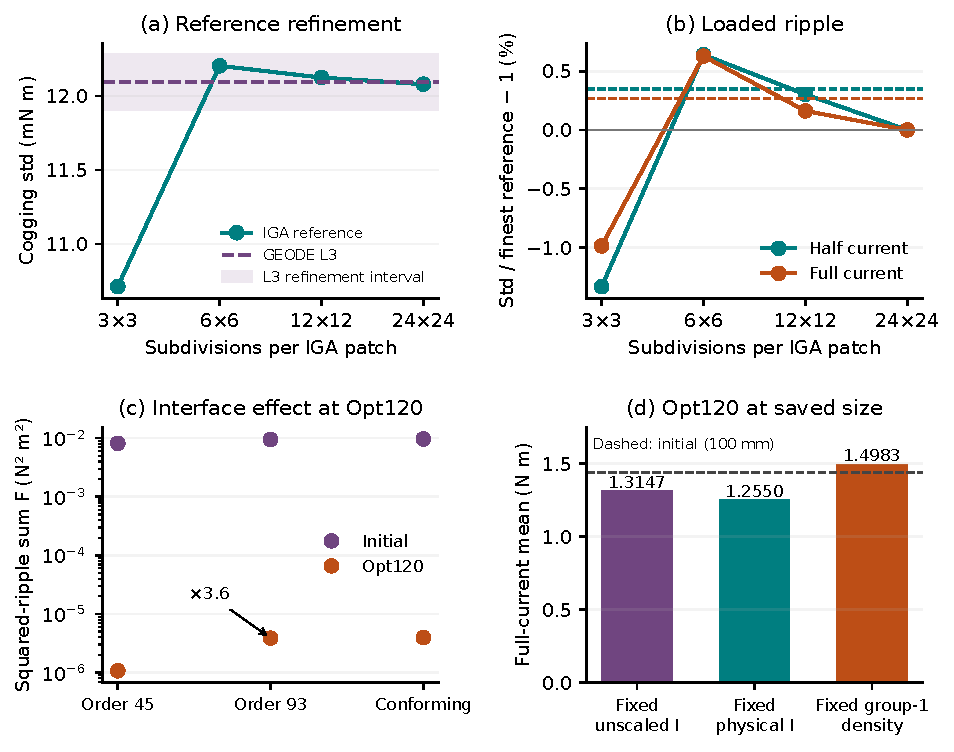
\includegraphics[width=\linewidth]{figures/refined-validation.pdf}
\caption{Reference and candidate validation from raw torque records.
(a) Independent IGA reference cogging refinement at order 45; the dashed
line is GEODE L3 and its shaded band uses Eq.~\eqref{eq:band}.
(b) Loaded standard deviation relative to the finest
reference at each current; circles are IGA, horizontal lines are GEODE L3.
The finest IGA point is zero by construction.
Panels (a,b) use the initial geometry and 20 angles; GEODE uses Arkkio,
with coupling torque checked separately. (c) Initial and Opt120 squared
ripple sums at L3 on fresh meshes and 20 angles, under fixed unscaled
current. Harmonic values use coupling torque; conforming values use
outer-band Arkkio. (d) Full-current mean at order 45 for Opt120 under
three current rules at its saved size (Appendix~\ref{sec:opt120-policy});
the dashed line is the initial mean at the initial size. All candidate
values use coupling torque.}\label{fig:validation}
\end{figure}

This agreement still concerns finite discretizations. The last cogging
increments approximately halve; extending that trend would put a limit
near 0.0120\,N\,m, an estimate without a bound. The last two half-current
standard-deviation increments are both about $-0.3\%$ and do not shrink;
we therefore leave its remaining error unestimated. The 0.10\% cogging
agreement is a comparison of finite-resolution values, not an accuracy
bound; neither refinement sequence is fully converged.
Tightening the reference Newton stopping threshold from $10^{-6}$ to
$10^{-14}$ changes the checked cogging torques by at most
$4.4\times10^{-8}$\,N\,m. GEODE retains straight-sided geometry, and the
high-field extrapolation of the iron law has not been varied in a paired
torque experiment. Neither cross-code agreement nor refinement proves
physical accuracy for the machine.

\subsection{The saved optimized design}\label{sec:opt120}
The saved reference design at iteration 120, denoted Opt120, includes
12 scalar parameters and ten grouped surface-control offsets. We evaluate
its full exported geometry on freshly generated meshes; simply moving
the finest initial mesh produces four inverted triangles. Its inner
air-gap band no longer has the annular area assumed by the full-band
Arkkio functional, so harmonic results here use coupling torque.
Conforming results use only outer-band Arkkio on the fresh exported mesh.
On the same L3, order-45 Opt120 field at full current, the outer-band and
coupling estimates differ by about $1.3\times10^{-4}$\,N\,m in mean and
$1.1\times10^{-5}$\,N\,m in standard deviation. This paired check supports
the estimator substitution at this resolution.
This estimator restriction is specific to these geometries; it does not
validate outer-band Arkkio on arbitrary moved meshes or stator offsets.

With the evaluation current held fixed in the unscaled geometry, raising
the transmitted order from 45 to 93 multiplies Opt120's $F$ by 3.6, from
$1.07\times10^{-6}$ to $3.86\times10^{-6}\,\mathrm{N^2\,m^2}$
(Fig.~\ref{fig:validation}c). The initial design's
$F$ rises by 16\%. Its ratio to Opt120 is consequently 7,631 at order 45,
2,454 at order 93 and 2,444 for conforming coupling. The full-current
Opt120 standard deviation rises from 0.00066 to 0.00164\,N\,m.
The large ripple reduction survives these checks, but its magnitude
depends strongly on the interface model: the order-93 change is about 96
times the last spatial-refinement increment of $F$
(Appendix~\ref{sec:opt120-policy}).

A possible explanation is that optimization against order 45 favors
cancellation within that truncated model. This is a conjecture, not an
ablation result: increasing the order raises full-current ripple but
lowers Opt120 cogging standard deviation from 0.00061 to 0.00035\,N\,m.
Appendix~\ref{sec:exp2-times} reports the corresponding coarse-to-validation
ratios at the designs selected in the optimization study.
Opt120 is also outside the fixed-size, fixed-physical-current problem of
Section~\ref{sec:optimization}: it shortens the stack from 100 to 80\,mm and
scales the radius by 1.0477, so its mean torque must be compared with the
initial motor only after both size factors and the current rule are fixed.
Appendix~\ref{sec:opt120-policy} gives those normalizations, a reproduction
comparison at the saved reference current, and the effect of angular
sampling at this low ripple.


\section{Forward-model controls}\label{sec:controls}
\begin{figure}[H]\centering
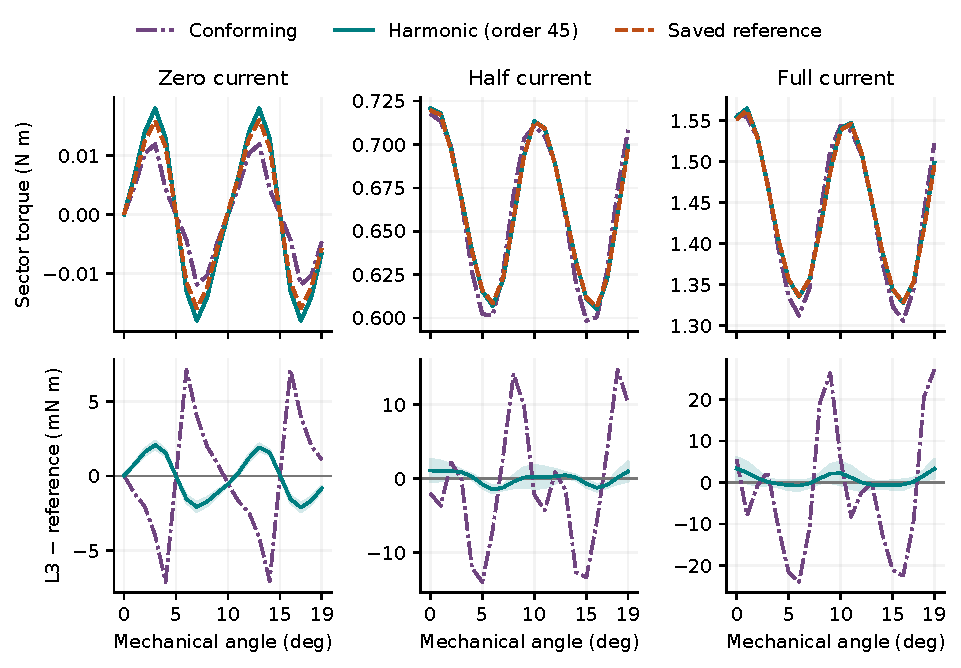
\includegraphics[width=\linewidth]{figures/coupling-waveforms.pdf}
\caption{Top: L3 torque for conforming and order-45 harmonic coupling,
compared with the saved reference. Bottom: each GEODE waveform minus the
reference; shading is the harmonic model's pointwise estimated refinement
interval from Eq.~\eqref{eq:band}. Each residual panel has its own vertical
scale, so compare residual magnitudes by their axis values, not by curve
height. All GEODE curves use Arkkio torque, so the paired difference changes the
coupling while holding the estimator fixed. The saved reference is coarse;
Section~\ref{sec:refinement} reports its refinement.}
\label{fig:waveforms}\end{figure}

The controlled changes in Table~\ref{tab:sensitivity} are too small to
explain the observed waveform gap at the tested settings. The near-zero
material difference has particularly little effect on torque despite its
6.66\% local reluctivity difference. This is a measured sensitivity of
the initial design and does not establish insensitivity after optimization.

\begin{table}[H]\centering\small
\caption{Maximum absolute torque change relative to the baseline at the
same mesh level, using conforming coupling and Arkkio torque. Entries
summarize the recorded angle/current subsets.}
\label{tab:sensitivity}
\begin{tabular}{p{.48\linewidth}ll}\toprule
Change & Levels & Max. $|\Delta T|$ (N\,m)\\\midrule
Reference low-field interpolation and clamp & L2, L3 & $2.1\times10^{-6}$\\
Relative Newton tolerance $10^{-12}$ vs $10^{-8}$ & L2; L3 full current & $7.3\times10^{-8}$\\
Exact winding areas vs mesh areas & L2 & $3.9\times10^{-4}$\\
Inner or outer half of the Arkkio band & L3 & $7.3\times10^{-5}$\\
\bottomrule\end{tabular}
\end{table}

In the recorded estimator study, single-circle Maxwell-stress estimates
vary more with the integration radius than the half-band Arkkio estimates.
The paired coupling-torque and half-band checks of
Section~\ref{sec:forward} avoid selecting a favorable radius. A
post-processing filter of the solved conforming field also gives
non-monotone ripple changes across the tested cuts and currents; it does
not replace a field solve with a truncated interface. The complete filter
results are retained in the accompanying forward-study records.

\section{Opt120: size, current policy and angular sampling}\label{sec:opt120-policy}
Between L2 and L3, changes in
$F$, normalized by L3, reach 1.36\% for the initial design and 2.71\%
for Opt120 across the three models on the exported mesh family; these increments are not error bounds.
For Opt120 at order 45, the successive L1--L2 and L2--L3 increases in $F$
are $3.05\times10^{-8}$ and $2.90\times10^{-8}$\,N$^2$\,m$^2$,
so they barely shrink and do not establish an asymptotic rate. An alternate
freshly constructed mesh family changes by 3.22\% for Opt120 from L2 to L3.
The $2.79\times10^{-6}$\,N$^2$\,m$^2$ interface effect is about
96 times the last export-mesh increment, despite this unresolved remainder.

Current policy changes Opt120's feasibility (Fig.~\ref{fig:validation}d). At L3 and order 45,
the initial full-current mean is 1.4433\,N\,m. Opt120 gives 1.3147\,N\,m
under fixed \emph{unscaled} current, 1.2550\,N\,m under fixed physical
current, and 1.4983\,N\,m under the reference's fixed group-1 density rule.
The first two are 8.9\% and 13.0\% below the initial mean; the density-rule
value is 3.8\% above it. These policy comparisons use the same Opt120
geometry, but comparisons with the initial motor also change size:
Opt120 shortens the stack from 100 to 80\,mm and has radial scale
$s=1.0477$, unscaled outer diameter 130.293\,mm and operating angle
$-11.646^\circ$ (Table~\ref{tab:parameters}). Every Opt120 torque carries
the explicit size factor $s^2L/(0.1\,\mathrm{m})=0.878175$.
Removing both size factors from the fixed-unscaled-current mean gives
1.4971\,N\,m, 3.7\% above the initial mean. Applying the same normalization
to fixed physical current gives 1.4291\,N\,m, 1.0\% below the initial mean;
the density-rule value becomes 1.7061\,N\,m, 18.2\% above it. Normalizing
only length to 100\,mm under fixed unscaled current gives 1.6434\,N\,m
(+13.9\%), retaining the radial factor $s^2=1.098$.
These algebraic normalizations separate the size factors from the current
rule; they are not reoptimized designs. Most of the saved-size deficit
therefore comes from the size factor, although the normalized
fixed-physical-current value remains lower.

A separate reproduction comparison uses the saved reference current at
each design, rather than fixed unscaled current. At Opt120, GEODE's
order-45 full-current mean is 1.4986\,N\,m versus 1.5000\,N\,m in the
saved arrays, but its standard deviation is $3.53\times10^{-4}$ versus
$1.76\times10^{-4}$\,N\,m, a factor of 2.0. The half-current values are
$5.53\times10^{-4}$ and $4.37\times10^{-4}$\,N\,m.
The largest pointwise difference across the two loaded currents is about
$2.1\times10^{-3}$\,N\,m. With this matched current policy and zero-current
values included (zero current is rule-independent and taken from the
fixed-current record), the initial-to-Opt120 objective ratios are 10,170 for
GEODE and 11,982 for the saved reference. The 7,631 ratio of
Section~\ref{sec:opt120} instead holds unscaled current fixed. Reference
refinement was run only at the initial design, so the cause of the Opt120
discrepancy remains unresolved.

Angular sampling becomes more consequential at this low ripple. Relative
to the 40-angle grid, the ten-angle Opt120 objective reads about 1.05\%
high at order 45 and 5.90\% low at order 93 on the fresh L3 mesh; the
conforming value reads 17.1\% low. The accompanying records retain shifted
20-angle grids and withheld currents 0.25 and 0.75. Candidate validation
must check these effects at the candidate, since initial-design agreement
alone would miss them. All 3,240 solve rows in the 18 successful records used for
these candidate comparisons stopped at tolerance.
Figure~\ref{fig:opt-waveforms} shows the full and mean-subtracted waveforms.

\begin{figure}[H]\centering
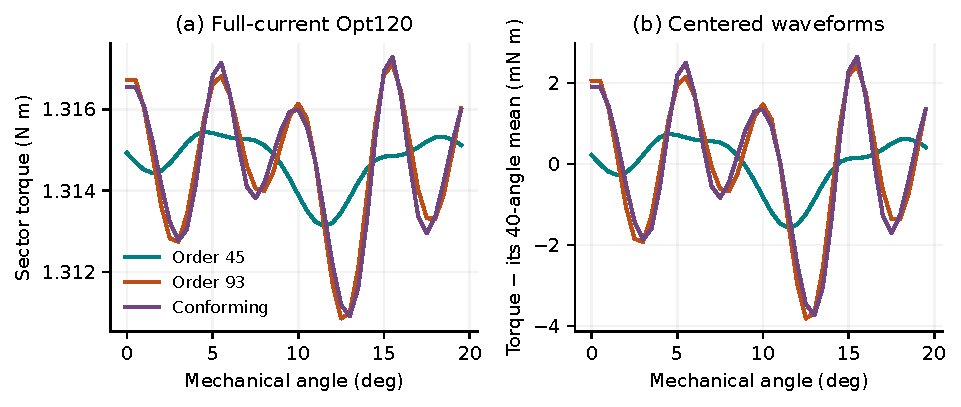
\includegraphics[width=\linewidth]{figures/opt120-waveforms.pdf}
\caption{Opt120 full-current torque on fresh L3 meshes at 40 angles,
with fixed unscaled current. Harmonic orders 45 and 93 use coupling torque;
conforming coupling uses outer-band Arkkio. Left: full torque, retaining
each model's mean. Right: each curve minus its own 40-angle mean.
The interface change mainly alters the resolved ripple.}
\label{fig:opt-waveforms}
\end{figure}

\section{Gradient verification details and derivative cost}\label{sec:cost}
\subsection*{Excitation rules}
In the scalar derivative study, fixed current means fixed peak current in
the unscaled geometry, so $J_g=12s_g I_q/|\Omega_g(X)|$ changes when a slot
changes area. The reference optimizer's rule, denoted \emph{fixed group-1
density}, sets $I_*\propto |\Omega_1(X)|s$, where $s$ is radial scale, with
the proportionality constant fixed at the initial design; the unscaled
geometry is evaluated and torque is multiplied by $s^2$, following the
reference. Both rules agree at the initial geometry but have different
derivatives. Group-2 density is not held fixed because the ratio of the two
winding areas can change. Rotor parameters MAG, MH and MW leave winding area
unchanged and therefore give identical derivatives under the two rules. The
fixed-size problem sets radial scale to one, making fixed physical and
unscaled current coincide.

\subsection*{Taylor remainders}
After removing duplicates and the analytic axial-length and radial-scale
cases, 530 of 592 loaded comparisons have an anchored quadratic-remainder
window spanning at least four decades in step size; 388 span at least five.
The window is the contiguous run where remainder/$h^2$ stays within a
factor of two of its value at $h=10^{-5}$\,m (or $10^{-2}$ degrees for
operating angle). Smaller gradients reach round-off sooner. An anchored-window diagnostic fails for the initial-design, full-current
conforming/fixed-density SW1 ripple cases at L0 and L1: at L0 the
remainder changes sign near the anchor, whereas at L1 remainder/$h^2$ is
still drifting there. Their widest quadratic windows span two decades. The nearly cancelling
zero-current mean is a weaker check: its best relative errors reach
$7.0\times10^{-4}$. Cogging standard-deviation errors are at most
$8.9\times10^{-7}$. Thus the loaded agreement does not describe every
zero-current derivative. Discrete derivative accuracy also does not imply
mesh convergence, as the next paragraph shows.

\subsection*{Model dependence of verified sensitivities}
The two model--estimator pairs give different ripple sensitivities even
at the same design (Fig.~\ref{fig:modelgradients}). At L2 and full fixed
current, the MAG ripple derivative is 1.28\,N\,m/m for harmonic/coupling
torque versus 1.94 for conforming/Arkkio at the initial design. At the
perturbed design the values are 0.75 and 1.87\,N\,m/m. These differences
persist under mesh refinement. At L3 the MAG pairs are 1.22 versus 1.87
at the initial design and 0.57 versus 1.67\,N\,m/m at the perturbed design.
In particular, the latter harmonic component changes appreciably even
though the box-scaled vector changes by only 1.19\% of its L2 norm;
the norm itself decreases by 0.19\%. Mean-torque
sensitivities agree more closely in the box-scaled comparison: the
Euclidean norm of the vector difference, divided by the conforming vector
norm, is 0.58\% and 0.66\% for the mean at the initial and perturbed
designs, versus 6.7\% and 10.2\% for ripple. The norm weights the largest
components most heavily: the initial SW2 and SW3 mean components differ
by 6.5\% and 16.5\% relative to conforming values.
At L3, the ripple gaps remain 6.58\% and 10.25\%, while each model
changes by 0.46--1.19\% from L2 to L3. The mean gaps fall to 0.16\%
and 0.26\%; the conforming model itself changes by 0.52--0.54\%.
The L2 mean gap is therefore comparable to spatial refinement, whereas
the ripple gap persists beyond the measured refinement increments. Because the
estimator changes with the model, this experiment measures their combined
effect; it does not isolate an interface-only derivative error or establish
which gradient is closer to the physical machine.

Discrete derivative accuracy also does not imply mesh convergence. In the
harmonic model, SW3 mean-torque sensitivities change sign between coarse
levels and their increments shrink with refinement; ripple gradients converge
more slowly than most mean gradients. The conforming/Arkkio SW2 mean
sensitivity is non-monotone across L0--L3 ($-46.5$, $-41.3$, $-44.4$,
$-47.2$\,N\,m/m), whereas harmonic/coupling torque approaches $-47.1$
from $-49.8$\,N\,m/m. Fresh-remesh checks of MW, SW1 and SW2 are limited
at small steps by changes in connectivity. The L2 MW mean-derivative fit
has relative gap $2.6\times10^{-6}$, but individual remeshed steps at
$h\geq10^{-4}$\,m scatter by about $6\times10^{-4}$. The largest L2 full-current
remeshed-versus-moved fitted discrepancy is 3.8\% for the SW1 ripple
derivative. These checks support the discrete chain rule while leaving
refinement of candidate designs necessary.

\begin{figure}[H]\centering
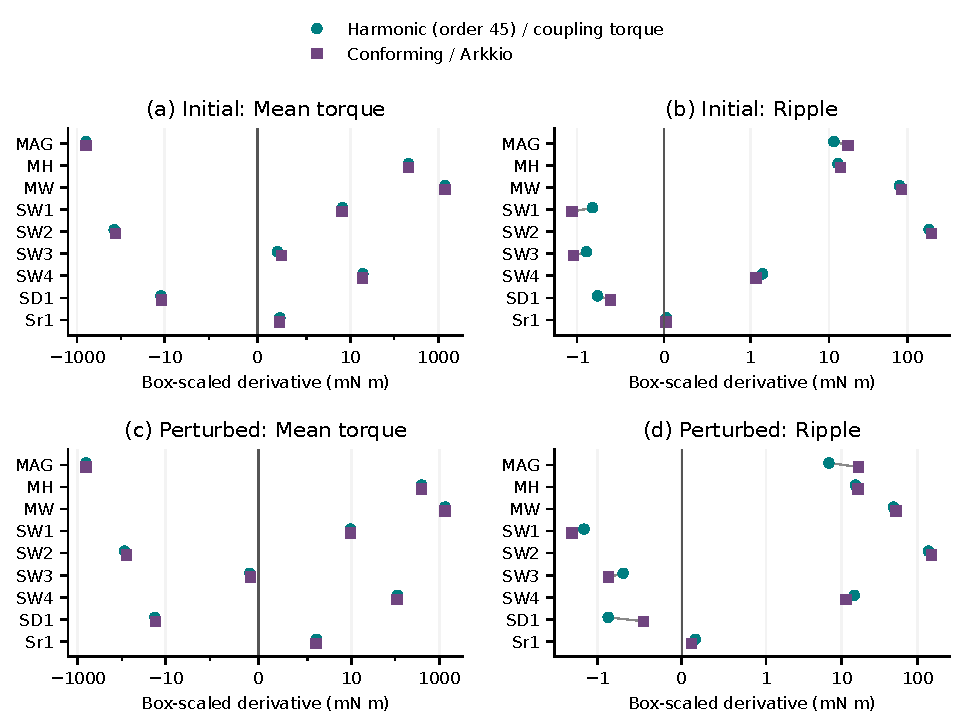
\includegraphics[width=\linewidth]{figures/model-gradients.pdf}
\caption{Full fixed-current sensitivities at L2, scaled by each geometric
parameter's reference box width $w_k$. Top: initial design; bottom:
perturbed design. L3 MAG values and refinement changes are given in the
text. Left: mean torque; right: standard deviation. The plotted
quantity $w_k\partial q/\partial p_k$ is a local sensitivity, not a finite
change across the box. Coupling and torque estimator both differ between
the two series. Gray segments join the two estimates for each parameter. Horizontal axes are symmetric-log, linear within
$\pm1$\,mN\,m. All nine widths, in mm, are 9, 10, 15, 4, 3, 1, 18, 70 and
1.5 in the displayed order.}\label{fig:modelgradients}
\end{figure}


The recorded timings use an Apple M3 Ultra with 28 cores, default solver
threading, and concurrent host load averaging 14--24. The effective thread
count was not pinned. A forward evaluation covers ten angles, starts from
zero, and warm-starts successive angles. The full gradient includes that
forward, ten torque adjoints, mesh derivatives and contractions for all
12 parameters and both aggregate objectives. Central differences use 24
forward sweeps, each warm-started from the base states, at step
$h=10^{-6}$ in each parameter's stored unit (m, degrees or dimensionless
scale), plus the shared base forward for a common starting point. Across
L0--L2, both couplings and tolerances $10^{-8}$ and $10^{-14}$, the full
gradient costs 1.13--1.20 forwards, whereas central differences cost
8.2--10.5 including the shared base solve (Fig.~\ref{fig:gradients}d and
Table~\ref{tab:cost}). Shape-map setup is a separate one-time cost of
these timings; the optimization study charges whole-run wall time, so it is
included there. These derivative timings concern one loaded host and are a
separate workload from the 1,640 forward validation solves of
Section~\ref{sec:forward}.

\begin{table}[H]\centering\small
\caption{Recorded harmonic-model cost at relative tolerance $10^{-14}$,
initial design and full current. Times are seconds for ten-angle sweeps;
FD includes the shared base sweep, and setup is a one-time shape-map cost.}
\label{tab:cost}\begin{tabular}{lrrrr}\toprule
Mesh & Forward & Forward + gradient & Base + FD & Setup\\\midrule
L0 & 0.664 & 0.748 & 6.997 & 0.011 \\
L1 & 3.174 & 3.658 & 32.811 & 0.041 \\
L2 & 12.702 & 14.644 & 129.390 & 0.222 \\
\bottomrule\end{tabular}

\end{table}

\section{Linear slotless screening control}\label{sec:slotless}
The stored slotless model has 24 distinct angles. Fitting
$T(\phi)=c_0+c_1\cos\phi+c_2\sin\phi$, with electrical angle $\phi=p\theta_r$, mechanical rotor angle $\theta_r$
and pole-pair count $p$, on alternate angles and
evaluating on the other twelve gives normalized held-out RMSE
$3.08\times10^{-10}$ and maximum error $6.82\times10^{-10}$, using the
recorded analytic-amplitude normalization. This is a locked-rotor angle sweep,
not synchronous operating ripple. For a fixed linear field operator and
sinusoidal sources, the field lies in a small basis of source responses;
a quadratic torque functional can contain only the corresponding finite
set of harmonics. The particular model needs just the three fitted
coefficients. This is an angular interpolation test at one geometry,
not a shape-gradient test or evidence of generalization across designs.

\section{Design points for derivative checks}\label{sec:parameters}
Table~\ref{tab:parameters} identifies the scalar derivative-study coordinates
and the saved Opt120 coordinates. Values are rounded for display; the accompanying records
retain full precision. The operating angle is stored in degrees and
converted to radians in the current equation. These coordinates describe
the scalar design space; the saved reference optimum additionally contains
surface-control offsets.
\begin{table}[H]\centering\small
\caption{Initial and interior perturbed design points for derivative
checks, alongside Opt120 for the forward validation. Lengths refer to the
unscaled geometry; surface-control offsets are retained in the data.}\label{tab:parameters}
\begin{tabular}{l>{\raggedright\arraybackslash}p{.28\linewidth}lrrr}\toprule
Parameter & Meaning & Unit & Initial & Perturbed & Opt120\\\midrule
MAG & Pole-axis iron depth above magnet & mm & 7.0000 & 6.5506 & 6.1011 \\
MH & Radial magnet height & mm & 7.0000 & 4.8722 & 2.7444 \\
MW & Magnet width & mm & 19.0000 & 19.8670 & 20.7340 \\
SW1 & Stator tooth width & mm & 4.0000 & 4.0309 & 4.0619 \\
SW2 & Slot-opening width & mm & 2.3000 & 1.6500 & 1.0001 \\
SW3 & Slot-opening depth & mm & 1.0000 & 0.7502 & 0.5004 \\
SW4 & Back-iron depth on slot axis & mm & 8.2500 & 6.8418 & 5.4336 \\
SD1 & Stator outer diameter & mm & 135.0000 & 132.6466 & 130.2931 \\
Sr1 & Slot-bottom fillet radius & mm & 1.0000 & 1.4999 & 1.9998 \\
LENGTH & Axial length & mm & 100.0000 & 90.0003 & 80.0005 \\
$\phi_0$ & Electrical current offset & $^\circ$ & 0.0000 & $-$5.8231 & $-$11.6463 \\
ScaleR & Radial similarity scale & 1 & 1.0000 & 1.0239 & 1.0477 \\
\bottomrule\end{tabular}

\end{table}

\setlength{\bibsep}{3pt}
\bibliographystyle{plainnat}
\bibliography{refs}
\end{document}
